% !Mode:: "TeX:UTF-8"

% Updated by Abraham Xiao, 20130608 XY511 11:25
% Updated by Abraham Xiao, 20130608 XY511 15:00
\chapter{绪论}\label{Introduction}
近年来,随着超大规模集成电路技术的飞速发展以及人们对更加高速、稳定的数字通信系统需求的不断增长,
通信系统和信号处理系统的复杂度也在日益增加。这种程度的发展让传统的系统设计方法显得捉襟见肘,更不用说
动态地分析系统设计中出现的各种问题。为此,研究人员在不断尝试新的、高效的设计分析工具---在电子计算机
日益普及的时代,计算机辅助的系统模拟方法 (Simulation) 正逐渐从实验室走向市场,被企业界认可。更高级的
系统仿真方法 (Emulation) 限于作者的研究时间和精力,将在工作展望部分进行适当阐述。
\par
通信系统的模拟,主要是通过数字计算机辅以相应的分析软件,对系统特性的一个或多个方面进行“模拟”,也就是
计算。通信系统模拟的研究人员的设想是,假如物理的(现实生活中的)通信系统的每一个要素都可以用一个数学模型
来表示,那么数字计算机将会“变身”成为一个完全虚拟的通信环境---只需要按照现实情况把各个要素连接起来。如
摘要中所述,这样纯粹的虚拟环境越来越受研究人员欢迎,很重要的一点是模型中的每一个参数可以根据需要随时进行
调整,调整后的结果也能很方便的观测到---这大大简化了用传统的方法逐步逼近最优参数的工作量。

\section{研究背景}\label{ResearchBackground}
最早的控制系统模拟可以追溯到20世纪50年代初期,电子计算机刚刚诞生的时候。由于使用的仍是模拟器件,
当时的计算机可被视为对一个连续系统的模拟.该连续系统由大量互相接在插线板上的模块构成,而这些模块,
分别代表了系统框图\upcite{ENIAC}上的不同部分。框图上的线性元件,诸如积分器、信号求和点以及放大器
均通过功率放大器来进行模拟。非线性元件,诸如限制器和一些非线性函数,则可以通过几个线性、非线性
元件的组合来表示。由以上推理可知,在数字通信领域,任何一个系统,无论它的特性是由常数或时变 (time
varying)参数的线性、非线性微分方程来表示,都能够被化简成一个框图 (block diagram),进而通过计算机
软件提供的组件搭接模拟。模拟的系统搭接好之后,根据给定输入信号(一称激励信号,exciting signal)的
不同,研究人员可以在输出端观测到系统的各种动态特性\upcite{Tranter1994}。
\par
从20世纪60年代开始,技术的进步让原本纯粹模拟 (analog) 的系统特性分析方法渐渐向数字化 (digital) 转移。
数字化的系统模拟架构由诸如连续系统建模程序 (Continuous System Modeling Program, CSMP)和其他一些面向
模块的编程语言搭建。这些编程语言通过一个部件、一个部件的分析方式来完成对模拟计算机的仿真。研究人员
开发出这些编程语言的最初动力是将繁杂的、模拟的分析方式升级成简单、方便的分析方式---用几行代码,就可以
将一堆框图所要传递的信息表示出来,结果还是一样的。上世纪60年代中叶,成套的电路级模拟软件诸如SPICE和
ECAP被开发出来,这些软件大大降低了系统分析中数值积分和信号流图中拓扑化简的工作量。从加州大学伯克利分校
电子工程和计算机科学系的主页上可以看到,经历了半个世纪,SPICE在教学中仍是极好的工具\upcite{Rabaey2013}。
\par
从20世纪60年代末到70年代初,离散时间系统和数字信号处理领域的发展带来了又一波数字方法的系统分析浪潮。
随之而来的分析软件有SYSTID,CSMP,CHAMP,LINK等等。这些软件中的部分在设计和分析卫星通信链路的时候发挥了
巨大的作用\upcite{Jeruchim2000}。
\par
从20世纪80年代开始,随着软件工程理论的不断推进,带有菜单的交互式系统分析软件如ICSSM,TOPSIM和ICS被开发出来。
这些软件让仿真从命令行窗口进入了图形化时代。
\par
自20世纪80年代中叶起,通信系统的模拟以及仿真在电子工程学科下作为一个独立的领域受到越来越多的关注。这些年
计算机的软硬件仍取得了很大的发展,并且再可预见的几十年里还有很大的发展空间。硬件方面,个人计算机已经成为
了一般研究人员的主流分析工具;软件方面,从20世纪90年代的BOSS,SPW,COSSAP等软件,到今天占据绝对多数的
MATLAB\upcite{MATLAB} (有几乎覆盖科研全领域的工具箱)\label{MATLABandItsToolbox}提供交互式用户友好图形化模拟仿真环境。
\section{章节安排}\label{ChapterArrangement}
本文主要研究了数字通信系统的建模和计算机模拟。引入的几个主要研究方法是,蒙特卡洛方法 (Monte Carlo method)、
准分析方法 (Quasi Analytical method)、仿射投影算法\upcite{Ozeki1984}(Affine Projection Algorithm, APA)。 本文对这几种方法在信道评估
领域做出了极为细致的比较。除此之外,本文也适当采用了其他一些方法,会随着行文逐渐展开,不一一赘述。
\par
作为一篇本科生毕业设计的学位论文,作者觉得还是很有必要阐述一些通信,尤其是数字通信领域的基础知识。
一是为了所有可能参考这篇文献的人行方便,二是为了巩固作者自身的学科基础---工程和科学领域什么东西
都能和数学沾点边,而牢固的数学基础又是做出优秀成果的有力保证。
\par
第二章介绍了数字通信系统模拟的背景知识。诸如常见信号的离散表示以及带通信号的低通表示。作为本文
研究的主要内容,信道的基本概念和几种常见的信道模型也做了一定的介绍。
\par
第三章讨论了仿射投影算法在自适应滤波 (Adaptive Filtering) 中的应用。从该算法的基础知识,到应用在
自适应滤波上的一些最基本的性能分析都有所讨论,
\par
第四章和第五章是本文的核心部分。第四章分析了整个信道评估方法设计的全过程,从信道建模到最后结果的
评估方案。并且构造了几种有效的机制对几种分析方法做了横向比较。
\par
第五章是结果阐述部分。对前几章提出的各种分析进行了MATLAB模拟计算,并依据行业惯例,绘制了若干张更加
直观的评价系统特性的图。
\par
第六章对全文所有工作进行了一个总结。然后对论文最终稿的成果进行了分析,列举出了几个可以从本文
继续延伸拓展研究的方向。

\chapter{背景知识}\label{FoundamentalKnowledge}
通常来说,系统可以被视为为了完成特定任务组合联结而成的几个部件\upcite{Ziemer1998}。信号则可被视为,
它通常是在时间维度上的一些量的集合。在通信领域用的信号一般是电压或者电流,本文实验中用的信号是随机信号,
由于不涉及实际意义,仅作分析方法是用,故不带单位。
\par
我们所期望模拟的现实生活中的信号,占绝大多数的是连续信号。但是,受限于数字计算机的物理特性,
在进行模拟的时候只有将模拟信号进行采样 (sampling) 和量化 (quantizing) 处理。
\section{连续和离散信号}\label{ContinuousandDiscreteSignal}
连续信号,顾名思义,就是在时间上是连续的信号。它的数学定义为一个以连续时间为自变量的实数或复数域函数。
在连续信号里,人们定义了几个十分基础的信号,例如单位阶跃信号 (unit step function)、单位脉冲信号 (unit
pulse signal)和 sinc 信号。这些信号从定义到推导到理论应用,在每一本《信号与系统》教材上都有所阐述,
因此本文不再赘述。
\par
离散信号与连续信号不同的地方在于,离散信号仅仅定义在一个或多个离散的时间点上。最常见的一种离散信号
获得方式是对连续信号进行等间隔采样$t = nT_{s}$,其中$n$为整数。
\par
\label{SamplingTheory}我们希望从数学上可以根据采样到的信号恢复出原信号(即采样前的信号,连续信号)。采样定理(一称奈奎斯特定理)
从理论上指出了最小的采样频率。根据采样定理,任意带宽为$W$的连续信号$s(t)$能够在采样后恢复成原信号的最小采样频率
为$f_{s} \geq 2W$采样每秒。满足条件的最小采样频率$f_{n} = 2W$采样每秒被称为奈奎斯特频率。因此,从理论上
可以看出,现实生活中的任何一个信号都可被以不低于奈奎斯特频率的采样频率采样,然后量化成离散信号。这样得到
的离散信号,在数字通信系统分析时,并不会比直接用原信号有任何失真,还降低了计算复杂度。
\section{带通信号的表示}
根据参考文献\upcite{Tranter1994},数字通信系统的两大基本理论分别为采样定理(见\ref{SamplingTheory}节)和欧拉定理。
欧拉定理将实数域和复数域通过公式$e^{ix} = \cos(x) + i\sin(x)$联接起来。式中$e$为自然对数的底,$i$为
% Need some labels here to make me thesis more formal.
虚数单位。作为一篇本科生学位论文,本文仍会用一定篇幅来阐述与之相关的概念和基础应用,为后文设计和验证
实验做铺垫。
\par
从教材和现实生活经验中我们知道,信号(相关讨论在\ref{ContinuousandDiscreteSignal}节)可以被视为
承载着特定信息的数学量。在实际应用中,数字信息承载信号 (digital information-bearing signal,以下简称信息信号) 通常
需要经过某种类型载波 (carrier) 的调制然后才进行传输。当信息信号的带宽远远小于载波频率时,信息信号就可以
被视为窄带带通信号 (narrowband bandpass signal,简称窄带信号)。我们将对后文需要用到的公式做一个推导,力求
获得最简形式。
\par
如前所述,当采样频率大于或等于奈奎斯特频率的时候,任意连续信号都可以用其等价的离散信号予以表示。这也就是说,
假设某带通连续信号的带宽为$B$,其载波频率为$f_{c}$,那么不失真的最小采样频率为$2 \times (f_{c}+B/2)$,依据为
前文\ref{SamplingTheory}推导的采样定理。当然,如果仅仅讨论带宽为$W$的低通信号,其奈奎斯特频率便只是$2W$。
由参考文献\upcite{Oppenheim2009}可知,对载波调制的信号和相应的系统做一定限制,它们就能被分别当做低通
的对象来进行处理。下面进行适度的公式推导,假设采用的为最常见的余弦调制。
\par
任意余弦调制后的信号$x(t)$可以表示为
\begin{equation}% \label{}
    x(t) ~=~ r(t)\cos[2\pi f_{c}t + \varphi(t)]
\end{equation}
上式简化后可以表示为
\begin{equation}% \label{}
    x(t) ~=~ Re[r(t)e^{j\phi(t)}e^{j2\pi f_{c}t}]
\end{equation}
其中$j$为虚数单位,$r(t)$为幅值调制 (amplitude modulation),$\varphi(t)$为信号的相位调制 (phase modulation),
$f_{c}$为调制用的余弦载波的频率。那么,分析后不难发现信号
\begin{equation}% \label{}
    v(t) ~=~ r(t)e^{j\varphi(t)}
\end{equation}
包含了信息信号$r(t)$的所有信息,并且经过傅里叶变换\upcite{Oppenheim1996} (Fourier Transform)后可以看出其
低通特性。上述方法通常被称为复数域低通特性或者是信号的复数包络检测。如果任意信号满足本章前述的窄带特性,
那么将调制后的带通信号$x(t)$处理为低通信号$v(t)$,然后作为信道分析的激励信号,会在计算上有很大的方便。
\par
我们利用三角函数的和差化积与积化和差公式\upcite{Oppenheim1996},对上面得到的公式进行进一步的分析,
可以得到
\begin{equation}% \label{}
    x(t) ~=~ x_{d}\cos(2\pi f_{c}t) - x_{q}\sin(2\pi f_{c}t)
\end{equation}
其中$x_{d}$与$x_{q}$分别为带通信号$x(t)$在正交的而为坐标轴上的两个分量 (In-Phase, Quadrature)。从参考文献
\upcite{Oppenheim2009}中可以得知,如果该带通信号$x(t)$的带宽$B$,也就是其两个分量的带宽$B$满足条件
$B \ll f_{c}$,那么$x(t)$的希尔伯特变化可以视为
\begin{equation}% \label{}
    \tilde{x}(t) ~=~ x_{d}\sin(2\pi f_{c}t) + x_{q}\cos(2\pi f_{c}t)
\end{equation}
进而信息信号$x(t)$的分析式可以表示为
\begin{equation}% \label{}
    x_{+}(t) ~=~ x(t) + j\tilde{x}(t) = [x_{d}(t) + jx_{q}(t)]e^{j2\pi f_{c}t}
\end{equation}
进而载波调制的信号$x(t)$可以表示为
\begin{equation} \label{CarrierModulatedSignal}
    x(t) ~=~ Re[x_{+}(t)] = Re[\tilde{x}(t)e^{j2\pi f_{c}t}]
\end{equation}
综合以上各式,信息信号$x(t)$的等价低通表示,或者说复数域包络检测定义为
\begin{equation}% \label{}
    \tilde{x}(t) ~=~ x_{+}e^{-j2\pi f_{c}t} = x_{d}(t) + jx_{q}(t)
\end{equation}

\section{\emph{M}维相移键控调制信号}
根据参考文献\upcite{Oppenheim2009,Oppenheim1996}中提供的信号分析方法,任意一个\emph{M}维相移键控调制信号
 (\emph{M-ary} Phase-Shift Keying Signal)可以表示为
 \begin{equation} \label{MaryPhaseShiftKeyingSignal}
    s(t) ~=~ A\cos[2\pi f_{c}t+\frac{2\pi}{M}(m-1)+\theta_{i}]
 \end{equation}
 其中$1 \leq m \leq M$,$0 \leq t \leq T$并且$\theta_{i}$是信号在发送端 (transmitter) 加上的相角 (phase angle)。
 公式\eqref{MaryPhaseShiftKeyingSignal}可以简化表示为
 \begin{equation}% \label{}
    s(t) ~=~ ARe\{e^{j[\frac{2\pi}{N}(m-1)+\theta_{i}]}e^{j2\pi f_{c}t}\}
 \end{equation}
 由公式\eqref{CarrierModulatedSignal}及参考文献\upcite{Oppenheim2009,Oppenheim1996}可知,复数形式的包络函数(包络检测获得)为
 \begin{equation}% \label{}
    \tilde{s}(t) ~=~ Ae^{j[\frac{2\pi}{M}(m-1)+\theta_{i}]}
 \end{equation}
 因此该包络函数的正交分量分别为
 \begin{equation}% \label{}
    x_{d}(t) ~=~ A\cos[\frac{2\pi}{M}(m-1)+\theta_{i}]
 \end{equation}
 和
 \begin{equation}% \label{}
    x_{q}(t) ~=~ A\sin[\frac{2\pi}{M}(m-1)+\theta_{i}]
 \end{equation}

 \section{\emph{M}维频移键控调制信号}
根据参考文献\upcite{Oppenheim2009,Oppenheim1996}中提供的信号分析方法,任意一个\emph{M}维频移键控调制信号
 (\emph{M-ary} Frequency Shift Keying Signal) 可以表示为
 \begin{equation}% \label{}
    x(t) ~=~ A\cos[2\pi(f_{c}+I_{m}\Delta f)t+\theta_{m}]
 \end{equation}
 或者其复数域表示
 \begin{equation}% \label{}
    x(t) ~=~ ARe\{e^{j2\pi f_{m}\Delta f}e^{j\theta_{m}e^{j2\pi f_{c}t}}\}
 \end{equation}
 其中$1 \leq m \leq M$,$\Delta f = \frac{1}{T}$。并且$\Delta f$是为了保证信号正交性的最小频率间隔。
 此外,还有$I_{m} = \frac{2m-1-M}{2}$。$\theta_{m}$表示的是每一个信号集中,信号的相位。
 \par
 由公式\eqref{CarrierModulatedSignal}及参考文献\upcite{Oppenheim2009,Oppenheim1996}可知,\emph{M}维频移键控调制信号
 的包络函数为
 \begin{equation}% \label{}
    \tilde{x}(t) ~=~ Ae^{j(2\pi f_{m}\Delta ft+\theta_{m})}
 \end{equation}
 可得其正交分量为
 \begin{equation}% \label{}
    x_{d}(t) ~=~ A\cos(2\pi I_{m}\Delta ft+\theta_{m})
 \end{equation}
 及
 \begin{equation}% \label{}
    x_{q}(t) ~=~ A\sin(2\pi I_{m}\Delta ft+\theta_{m})
 \end{equation}

 \section{通信系统中的滤波}
 通信系统中的滤波主要用来选择特定的信号以及减轻或消除干扰 (interference) 和噪声 (noise)。一个理想的滤波器
 ,在其通带(也就是进行滤波的频段)传递函数的幅值 (magnitude) 是恒定不变的一个值;在其阻带,传递函数的幅值为
 0.理想滤波器的中频带增益为1,其相位为关于频率的线性函数\upcite{Ziemer1998}。
 \par
 在对数字通信系统进行模拟的时候,带通信号的滤波通常都简化为对其复数域的包络函数进行处理。带通滤波器
 一般也等价成低通滤波器方便分析。前文\ref{MATLABandItsToolbox}节中分析过,在MATLAB软件中,各式各样的滤波器
 都只需要几个参数,诸如通带 (passband)、阻带 (stopband)和这些频带中的公差 (tolerances)就可以确定下来。
 在MATLAB中最常见的描述方式为传递函数---分子和分母都是多项式。


 \chapter{仿射投影自适应滤波器}
自适应滤波器在统计信号处理中占有相当重要的地位。当需要处理统计特性未知 (unknown statistics)
或者根本就不固定环境中产生的信号时,自适应滤波器相比用传统方法设计的固定滤波器 (fixed filters) 在
处理结果的精度和可靠性上有显著的改善,因此采用自适应而非传统滤波器在这些环境中是极富吸引力的。
进一步来说,虽然从理论上来看自适应滤波器的处理速度没有传统的快,但是经过多年的发展,目前最先进的
自适应滤波器已经完全不输传统滤波器,在处理速度方面;在系统的复杂度方面,自适应滤波器由于其结构
特性,略逊一筹也是不争的事实。从自适应滤波器诞生的那一天起,越来越多的实际应用中可以看到它的
身影。现如今,应用领域已包括诸如通信中的雷达和声呐,控制领域的各种新型控制器、地震的预测以及生物医学工程
领域的医学图像分析、病情诊断和预测等。
\par
本章主要讨论了仿射投影算法的数学基础和其在自适应滤波器中的应用\upcite{Haykin2002}。滤波器的自适应特性 (adaptation) 是通过
根据输入量(在通信系统中为输入信号)的变化来不断调整其自由参数 (free parameters) 也即其传递函数自变量的
系数,来获得的。然而,这样一种方式,却使得自适应滤波器成了一种非线性器件。所以,当我们说自适应滤波器
是一种线性器件的时候,我们是如下定义的:自适应滤波器的输入输出映射满足叠加定理,当且仅当在每一个瞬时,
滤波器的各个参数均为定值的时候。
\par
\section{仿射投影自适应滤波器的建立}
从数学角度上讲,设计一个基于仿射投影算法的自适应滤波器,就是一个在有多重限定条件的前提下
试图寻找最优解的过程。从下文开始我们慢慢讨论。
\par
试图将权重矢量增量的平方欧几里得范数最小化,我们可以得到下式
\begin{equation} \label{MinimizeSquaredEuclideanNorm}
    \delta\hat{\mathbf{w}} ~=~ \hat{\mathbf{w}}(n+1) - \hat{\mathbf{w}}(n)
\end{equation}
其$N$维限定条件是
\begin{equation} \label{SetOfNConstraints}
    d(n-k) ~=~ \hat{\mathbf{w}}^{H}(n+1)\mathbf{u}(n-k)\quad for\quad k = 0,1,...,N-1
\end{equation}
对于式\eqref{SetOfNConstraints}我们要求,也可以说成假设$N$要小于输入数据空间的维度,即$M$。输入空间
在这里也就是权重空间 (weight space) 。
\par
在这样一种$N$维的限定条件下,当$N = 1$时,就变成了归一化最小均方滤波器 (Normalized Least Mean Square Filter,简称
NLMS Filter)。因此,我们可以将限定条件的数量$N$视为,基于仿射投影算法的自适应滤波器的\emph{阶数} (order)。
\par
根据参考文献\upcite{Haykin2002}的附录C (pp 799-801)中描述的\emph{多重约束条件下拉格朗日乘子}的计算法则,
我们将方程\eqref{MinimizeSquaredEuclideanNorm}和\eqref{SetOfNConstraints}组合起来建立仿射投影自适应滤波器
的代价函数
\begin{equation} \label{AffineProjectionFilterCostFunction}
    \mathbf{J}(n) ~=~ \|\hat{\mathbf{w}}(n+1) - \hat{\mathbf{w}}(n)\|^{2} + \sum^{N-1}_{k=0}Re[\lambda^{*}_{k}(d(n-k)-\hat{\mathbf{w}}^{H}(n+1)\mathbf{u}(n-k))]
\end{equation}
在代价函数\eqref{AffineProjectionFilterCostFunction}中,$\lambda_{k}$是关于多重限定条件的拉格朗日乘子。
为了在后面中的描述简便起见,我们接着引入如下定义,
\begin{itemize}
  \item 一个$N$行$M$列的数据矩阵 (data matrix),其埃尔米特转置 (Hermitian transpose) 定义为
  \begin{equation}\label{NbyMDataMatrix}
    \mathbf{A}^{H} ~=~ [\mathbf{u}(n),\mathbf{u}(n-1),...,\mathbf{u}(n-N+1)]
  \end{equation}

  \item 一个$N$行$1$列期望响应矢量 (desired response vector),其埃尔米特转置定义为
  \begin{equation}\label{NbyOneDesiredResponseVector}
    \mathbf{d}^{H}(n) ~=~ [d(n),d(n-1),...,d(n-N+1)]
  \end{equation}

  \item 一个$N$行$1$列的拉格朗日矢量 (Lagrange vector),其埃尔米特转置定义为
  \begin{equation}% \label{}
    \boldsymbol{\lambda}^{H} ~=~ [\lambda_{0},\lambda_{1},...,\lambda_{N-1}]
  \end{equation}

\end{itemize}
将上述定义好的矩阵代入方程\eqref{AffineProjectionFilterCostFunction}中,一个简化后更加紧凑的代价函数
为
\begin{equation}% \label{}
    \mathbf{J}(n) ~=~ \|\hat{\mathbf{w}}(n+1)-\hat{\mathbf{w}}(n)\|^{2} +
    Re[(\mathbf{d}(n)-\mathbf{A}(n)\hat{\mathbf{w}}(n+1))^{H}\boldsymbol{\lambda}]
\end{equation}
为了求极值,我们用参考文献\upcite{Haykin2002}的附录B (pp 794-798)中给出的关于复数域矢量求微分的方法,
对代价函数$\mathbf{J}(n)$求关于权重矢量$\hat{\mathbf{w}}(n+1)$的导数,有
\begin{equation}% \label{}
    \frac{\partial\mathbf{J}(n)}{\partial\hat{\mathbf{w}}^{*}(n+1)} ~=~
    2(\hat{\mathbf{w}}(n+1)-\hat{\mathbf{w}}(n)) - \mathbf{A}^{H}(n)\boldsymbol{\lambda}
\end{equation}
将上式右边置为$0$,我们可以得到等式
\begin{equation}\label{DerivativeofCostFunction}
    \delta\hat{\mathbf{w}}(n+1) ~=~ \frac{1}{2}\mathbf{A}^{H}\boldsymbol{\lambda}
\end{equation}
为了讨论和求解的需要,我们想办法从方程\eqref{DerivativeofCostFunction}中消去拉格朗日矢量$\lambda$。
因此,我们首先利用方程\eqref{NbyMDataMatrix}和\eqref{NbyOneDesiredResponseVector}将最开始的
$N$维限定条件集重写为等价的形式,
\begin{equation} \label{EliminateTheLagrangeVector}
    \mathbf{d}(n) ~=~ \mathbf{A}(n)\hat{\mathbf{w}}(n+1)
\end{equation}
将方程\eqref{DerivativeofCostFunction}两边同时乘以$\mathbf{A}(n)$,然后利用方程\eqref{MinimizeSquaredEuclideanNorm}
和\eqref{EliminateTheLagrangeVector}消去更新后的权重矢量$\hat{\mathbf{w}}(n+1)$得到
\begin{equation}\label{EliminateTheUpdatedWeightVector}
    \mathbf{d}(n) ~=~ \mathbf{A}(n)\hat{\mathbf{w}}(n) + \frac{1}{2}\mathbf{A}(n)\mathbf{A}^{H}(n)\boldsymbol{\lambda}
\end{equation}
从上式\eqref{EliminateTheUpdatedWeightVector}我们可以推出如下结论:
\begin{itemize}
  \item 矢量$\mathbf{d}(n)$和$\mathbf{A}(n)\hat{\mathbf{w}}(n)$的差,是一个以迭代次数 (iteration)为自变量的
  $N$行$1$列误差矢量 (error vector)
  \begin{equation} \label{NbyOneErrorVector}
    \mathbf{e}(n) ~=~ \mathbf{d}(n)-\mathbf{A}(n)\hat{\mathbf{w}}(n)
  \end{equation}

  \item 矩阵$\mathbf{A}(n)\mathbf{A}^{H}(n)$的乘积是一个$N$行$N$列的矩阵,我们将其逆矩阵记作
  $(\mathbf{A}(n)\mathbf{A}^{H}(n))^{-1}$
\end{itemize}
有了以上简化的表示,我们解方程\eqref{EliminateTheUpdatedWeightVector}求拉格朗日矢量,
\begin{equation}% \label{}
    \boldsymbol{\lambda} ~=~ 2(\mathbf{A}(n)\mathbf{A}^{H}(n))^{-1}\mathbf{e}(n)
\end{equation}
将解得的拉格朗日矢量代入方程\eqref{DerivativeofCostFunction},我们可以得到权重矢量的最优增量,
其表示形式为,
\begin{equation}\label{OptimumChangeInWeightVector}
    \delta\hat{\mathbf{w}}(n+1) ~=~ \mathbf{A}^{H}(n)\mathbf{A}(n)\mathbf{A}^{H}(n)^{-1}\mathbf{e}(n)
\end{equation}
最后,也可以说是在基于仿射投影算法的自适应滤波器设计中最重要的一步,就是我们需要控制好
每一步权重矢量的迭代,使其尽可能保证在一个方向上\upcite{Ozeki1984} (keep the same direction)。
为了尽可能的实现这一目标,我们向方程\eqref{OptimumChangeInWeightVector}中引入步长参数$\tilde{\mu}$
(step-size parameter),进而得到新的方程
\begin{equation}% \label{OptimumChangeInWeightVector}
    \delta\hat{\mathbf{w}}(n+1) ~=~ \tilde{\mu}\mathbf{A}^{H}(n)\mathbf{A}(n)\mathbf{A}^{H}(n)^{-1}\mathbf{e}(n)
\end{equation}
将获得的每一步迭代的权重矢量增量代入其定义式(也就是其每步迭代的递推公式)\eqref{MinimizeSquaredEuclideanNorm}
,并进行整理,可以得到
\begin{equation}\label{DesiredUpdateEquationForAPAFilter}
    \hat{\mathbf{w}}(n+1) ~=~
    \hat{\mathbf{w}}(n) +
    \tilde{\mu}\mathbf{A}^{H}(n)\mathbf{A}(n)\mathbf{A}^{H}(n)^{-1}\mathbf{e}(n)
\end{equation}
这也就是最终我们利用基于仿射投影算法的自适应滤波器,在数字通信系统中进行信号处理的基本公式
\upcite{Ozeki1984,Haykin2002}。


\section{仿射投影运算}
由参考文献上的描述\upcite{Haykin2002}可得,迭代后的权重矢量$\hat{\mathbf{w}}(n+1)$是迭代前权重矢量
$\hat{\mathbf{w}}(n)$经过仿射投影运算的结果。为了得到仿射投影算子,我们将方程\eqref{NbyOneErrorVector}
代入方程\eqref{DesiredUpdateEquationForAPAFilter}可得,
\begin{equation}
\label{AffineProjectionOperator}
\begin{split}
    \hat{\mathbf{w}}(n+1)& ~=~ [\mathbf{I}-\tilde{\mu}
    \mathbf{A}^{H}(n)(\mathbf{A}(n)\mathbf{A}^{H}(n))^{-1}
    \mathbf{A}(n)]\hat{\mathbf{w}}(n) \\
    & \quad~~+ \tilde{\mu}\mathbf{A}^{H}(n)(\mathbf{A}(n)\mathbf{A}^{H}(n))^{-1}
    \mathbf{d}(n)
\end{split}
\end{equation}
其中$\mathbf{I}$为单位矩阵。由上式\eqref{AffineProjectionOperator}为了便于描述,定义投影算子 (projection operator)
如下:
\begin{equation}\label{ProjectionOperator}
    \mathbf{P}~=~\mathbf{A}^{H}(n)(\mathbf{A}(n)\mathbf{A}^{H}(n))^{-1}
    \mathbf{A}(n)
\end{equation}
对方程\eqref{ProjectionOperator}简单分析不难发现,$\mathbf{P}$由数据矩阵$\mathbf{A}(n)$
唯一确定。所以,对确定好了的$\tilde{\mu}$,$\mathbf{A}(n)$和$\mathbf{d}(n)$,互补投影算子
(complement projector)~$[\mathbf{I}-\tilde{\mu}\mathbf{P}]$作用在前一个权重矢量$\hat{\mathbf{w}}(n)$
上,产生新的权重矢量$\hat{\mathbf{w}}(n+1)$。最为重要的是,由于方程\eqref{AffineProjectionOperator}
中第二项的存在,也就是$\tilde{\mu}\mathbf{A}^{H}(n)(\mathbf{A}(n)\mathbf{A}^{H}(n))^{-1}\mathbf{d}(n)$,
使得互补投影算子成为了仿射投影算子而非简简单单的一个投影算子。
\par
在参考文献\upcite{Haykin2002}的第八章中(pp 385-429)谈到,对于各种最小均方算法,我们可以证明,
当$N$小于$M$时,矩阵
$\mathbf{A}^{H}(n)(\mathbf{A}(n)\mathbf{A}^{H}(n))^{-1}$可以被视为数据矩阵$\mathbf{A}(n)$的
伪逆(pseudoinverse)矩阵。用符号$\mathbf{A}^{+}(n)$来表示该伪逆矩阵,进一步将递推方程\eqref{AffineProjectionOperator}
简化表示为
\begin{equation}\label{SimplifiedAffineProjectionOperator}
    \hat{\mathbf{w}(n)}~=~[\mathbf{I}-\tilde{\mu}\mathbf{A}^{+}(n)\mathbf{A}(n)]
    \hat{\mathbf{w}}(n) + \tilde{\mu}\mathbf{A}^{+}(n)\mathbf{d}(n)
\end{equation}
至此,基于仿射投影算法的自适应滤波器递推公式的相关已全部讨论。当然,参考文献\upcite{Haykin2002}中
做了这样一个总结---“正是由于递推公式\eqref{SimplifiedAffineProjectionOperator}的定义,我们可以很直观
地将基于仿射投影算法的自适应滤波器视作,介于归一化最小均方滤波器和递归最小均方滤波器之间的一种滤波器,
就计算复杂度(computational complexity)和性能(performance)两方面来说。”

\section{仿射投影自适应滤波器的稳定性分析}
作出假设,即本文讨论的基于仿射投影算法的自适应滤波器的本质数学模型为多重回归模型(multiple regression model),
由上节讨论和参考文献\upcite{Haykin2002}的最小均方滤波器部分(pp 320-327)可知,模型的数学表达式可以为,
\begin{equation}\label{MultipleRegressionModel}
    \mathbf{d}(n) ~=~ \mathbf{w}^{H}\mathbf{u}(n)+ \mathbf{\nu}(n)
\end{equation}
在方程\eqref{MultipleRegressionModel}中,$\mathbf{w}$为模型的未知参数矢量,$\nu(n)$为加性干扰,
在归一化最小均方滤波器中,估测权重矢量(tap-weight vector)是通过该滤波器数学模型后,计算得到的对
真实$\mathbf{w}$的一个估计。因此可以定义真实值和估测值之间的误差(mismatch)一个专门的矢量---权重误差矢量
(weight-error vector)如下,
\begin{equation}\label{WeightErrorVector}
    \boldsymbol{\varepsilon}(n) ~=~ \mathbf{w}~-~\hat{\mathbf{w}}(n)
\end{equation}
再由归一化最小均方滤波器的递推方程\upcite{Haykin2002}
\begin{equation}\label{DesiredRecursionForNLMSFilter}
    \hat{\mathbf{w}}(n+1)~=~\hat{\mathbf{w}}(n)+\frac{\tilde{\mu}}{\|\mathbf{u}(n)^{2}\|}
    \mathbf{u}(n)\mathbf{e}^{*}(n)
\end{equation}
两式\eqref{WeightErrorVector}、\eqref{DesiredRecursionForNLMSFilter}相减,得
\begin{equation}\label{UpdatedWeightErrorVector}
    \boldsymbol{\varepsilon}(n+1)~=~\boldsymbol{\varepsilon}(n)-
    \frac{\tilde{\mu}}{\|\mathbf{u}(n)^{2}\|}\mathbf{u}(n)\mathbf{e}^{*}(n)
\end{equation}
在参考文献\upcite{Haykin2002,Sankaran2000,Sankaran2000A}中提到,设计归一化最小均方滤波器的一个核心思想便是
让估测权重矢量在每一次$n$至$n+1$的迭代 (iteration)中,尽可能达到最小值。而这样一种设计的实现,而这样一种最小化的
设想,却又受制于迭代本身。受上述过程的启发,我们不难想到用均方差(mean square deviation)来作为最小方差滤波器
稳定性的评价标准。
\begin{equation}\label{MeanSquareDeviation}
    \mathscr{D}(n)~=~E[\|\boldsymbol{\varepsilon}(n)\|^{2}]
\end{equation}
至此,对基于仿射投影算法的自适应滤波器稳定性分析的准备工作告一段落。现在正式开始分析。
\par
因为仿射投影滤波器也归纳在最小均方滤波器类别下,所以同该滤波器一样,我们对其的稳定性分析以
均方差$\mathscr{D}(n)$为评价标准,均方差的定义在式\eqref{MeanSquareDeviation}。用含有未知权重矢量
(unknown weight vector)的多重回归模型方程减去方程\eqref{DesiredUpdateEquationForAPAFilter},我们
可以得到下式
\begin{equation}% \label{}
    \boldsymbol{\varepsilon}(n+1)~=~\boldsymbol{\varepsilon}(n)-
    \tilde{\mu}\mathbf{A}^{H}(n)(\mathbf{A}(n)\mathbf{A}^{H}(n))^{-1}
    \mathbf{e}(n)
\end{equation}
将上述权重误差矢量的迭代公式代入$\mathscr{D}(n)$的定义中,对得到的式子进行重排和化简,有
\begin{equation}
\label{UpdatedMeanSquareErrorDefinition}
\begin{split}
\mathscr{D}(n+1)-\mathscr{D}(n) & ~=~ \tilde{\mu}E[\mathbf{e}^{H}(n)(\mathbf{A}(n)\mathbf{A}^{H}(n))^{-1}\mathbf{e}(n)]\\
& \quad~~-2\tilde{\mu}E\{Re[\boldsymbol{\xi}^{H}_{u}(n)(\mathbf{A}(n)\mathbf{A}^{H}(n))^{-1}\mathbf{e}(n)]\}
\end{split}
\end{equation}
其中
\begin{equation}
%\label{}
    \boldsymbol{\xi}_{u}(n)~=~\mathbf{A}(n)(\mathbf{w}-\hat{\mathbf{w}}(n))
\end{equation}
为非干扰误差向量(undisturbed error vector)。从方程\eqref{UpdatedMeanSquareErrorDefinition}中可以比较明显地
看出均方差$\mathscr{D}(n)$随着$n$的单调(monotonically)增加而单调减少---假定步长参数$\mu$满足条件
\begin{equation}
\label{}
    0 < \tilde{\mu} < \frac{2E\{Re[\boldsymbol{\xi}^{H}_{u}(n)(\mathbf{A}(n)\mathbf{A}^{H}(n))^{-1}\mathbf{e}(n)]\}}
    {E[\mathbf{e}^{H}(n)(\mathbf{A}(n)\mathbf{A}^{H}(n))^{-1}\mathbf{e}(n)]}
\end{equation}
同样不难发现,对于上式,归一化最小均方滤波器的$\tilde{\mu}$限定条件\upcite{Haykin2002}(pp 324-325)是其一个特例。
再对方程\eqref{UpdatedMeanSquareErrorDefinition}进行求导分析,得到最优步长(optimal step-size)的数学定义如下,
\begin{equation}
\label{AffineProjectionAdaptiveFilterOptimalStepSize}
    \tilde{\mu}_{opt}~=~\frac{E\{Re[\boldsymbol{\xi}^{H}_{u}(n)(\mathbf{A}(n)\mathbf{A}^{H}(n))^{-1}\mathbf{e}(n)]\}}
    {E[\mathbf{e}^{H}(n)(\mathbf{A}(n)\mathbf{A}^{H}(n))^{-1}\mathbf{e}(n)]}
\end{equation}
由上式已经可以得出足够多可用的信息,但是我们利用参考文献\upcite{Haykin2002,Sankaran2000,Sankaran2000A}中提到
的几条假设,并对其在本节的讨论中做出扩展,是我们可以在更加细小的范围内讨论$\tilde{\mu}_{opt}$,以便看出规律。
为了叙述得更加清楚,做出的假设(assumption)描述采用英文,即对参考文献中的假设做出适当修改后直接引用。
\begin{itemize}
  \item \textbf{Assumption I.}\quad \emph{F对于每一次的迭代, 该矩阵 $\mathbf{A}(n)\mathbf{A}^{H}(n)$}逆的波动大小, 作为
  $\tilde{\mu}_{opt}$的分子和分母, 可以小到忽略不计。进而将 $\tilde{\mu_{opt}}$ 简化为
  \begin{equation}
  % \label{}
    \hat{\mu}_{opt}~\approx~\frac{E\{Re[\boldsymbol{\xi}^{H}_{u}(n)\mathbf{e}(n)]\}}
    {E[\|\mathbf{e}(n)\|^{2}]}
  \end{equation}


  \item \textbf{Assumption II.} \quad \emph{非干扰误差矢量 $\boldsymbol{\xi}_{u}(n)$ 与干扰误差(噪声)矢量不相关}
  \begin{equation}
  % \label{}
    \boldsymbol{\nu}^{H}(n)~=~[\nu(n),\nu(n-1),...,\nu(n-N+1)]
  \end{equation}

  \item \textbf{Assumption III.} \quad \emph{输入信号 $u(n)$ 的频谱,在比每一个权重误差矢量$\boldsymbol{\varepsilon}(n)$所占带宽还要宽的
  区间内,都是平坦的。 据此我们可以做出以下近似}
  \begin{equation}
  \begin{split}
  % \label{}
    E[\xi^{2}_{u}(n)] & ~=~ E[|e^{T}(n)\mathbf{u}(n)|^{2}]\\
    & ~\approx~E[\|\boldsymbol{\varepsilon}(n)\|^{2}]E[u^{2}(n)]\\
    & ~=~\mathscr{D}(n)E[u^{2}(n)]
  \end{split}
  \end{equation}


\end{itemize}
应用以上三条假设,对方程\eqref{AffineProjectionAdaptiveFilterOptimalStepSize}进行化简,有
\begin{equation}
\begin{split}
% \label
\tilde{\mu}_{opt} & ~=~ \frac{E[\|\boldsymbol{\xi}_{u}(n)\|^{2}]}
    {E[\|\mathbf{e}(n)\|^{2}]}\\[15pt]
    & ~=~ \frac{\displaystyle{\sum^{N-1}_{k=0}}E[|\xi_{u}(n-k)|^{2}]}
    {\displaystyle{\sum^{N-1}_{k=0}}E[|e(n-k)|^{2}]}\\[15pt]
    & ~\approx~ \frac{\displaystyle{\sum^{N-1}_{k=0}}\mathscr{D}(n-k)E[|u(n-k)|^{2}]}
    {\displaystyle{\sum^{N-1}_{k=0}}E[|e(n-k)|^{2}]}
\end{split}
\end{equation}

\chapter{信道评估方法设计}
评价数字通信系统的各项指标中,接收到的信号与发送的信号之间出错的概率(即Bit Error Rate,BER~误码率 )是一项很重要也广泛被使用的评价指标。用蒙特卡洛方法进行通信系统信道评估,要点在于设计好一个大小为
$M$的字母表(或者其他你想要进行测试的数据,比如二进制数据报)作为发送信号(即系统的输入信号)。参考文献
\upcite{Tranter1994}中指出通常设计的字母表大小为$2^{k}$,这是由电子计算机的特性决定的。
\par 而计算误码率的通常方法是任意多次取任意长(由准确性考虑应当取得较长,视$M~=~2^{k}$大小而定)的接收信号(即系统的输出信号),
计算其平均的出错次数。其数学叙述大体如下:假设$N$为输入信号的数据量($N$个二进制数),$n(N)$为观测到的错误数,则出错概率$p$
定义为$p ~=~ \displaystyle{\lim_{N\rightarrow\infty}}\frac{n(N)}{N}$。对于前述的当字母表的大小$M=2$的时候,一个专有的名称为比特差错概率(误码率)。
\par
本章和第五章所讨论的数字通信系统,其模型简化为
\begin{figure}[htbp]% \label{}
  % Requires \usepackage{graphicx}
  \centering
  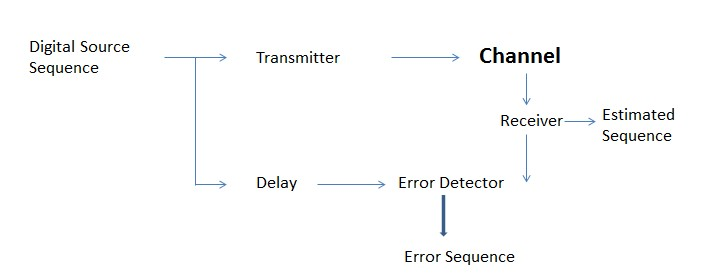
\includegraphics[scale=0.6]{SystemBlockDiagram.jpg}\\
  \caption{本文分析采用的系统框图} \label{CommunicationSystemBlockDiagram}
\end{figure}


\section{蒙特卡罗方法}
蒙特卡罗信道评估方法\upcite{Tranter1994,Ziemer1998}是基于统计学方法的,对真实通信系统的一种模拟。蒙特卡罗方法的核心在于建立真实 通信系统尽可能准确
的数学模型,然后依据模型进行推理、演算。最为常见的模型建立方法是框图法---一个例子如图\ref{CommunicationSystemBlockDiagram}。
根据任务要求,可以设计出类型相似但实际差别很大的框图出来\upcite{Tranter1994,Ziemer1998,Haykin2002}。如图\ref{EvolutionofMonteCarloSimulation}
和图\ref{BlockDiagramofReverseRadioLinkSimulatio}所示。
\begin{figure}
[htbp]
\centering
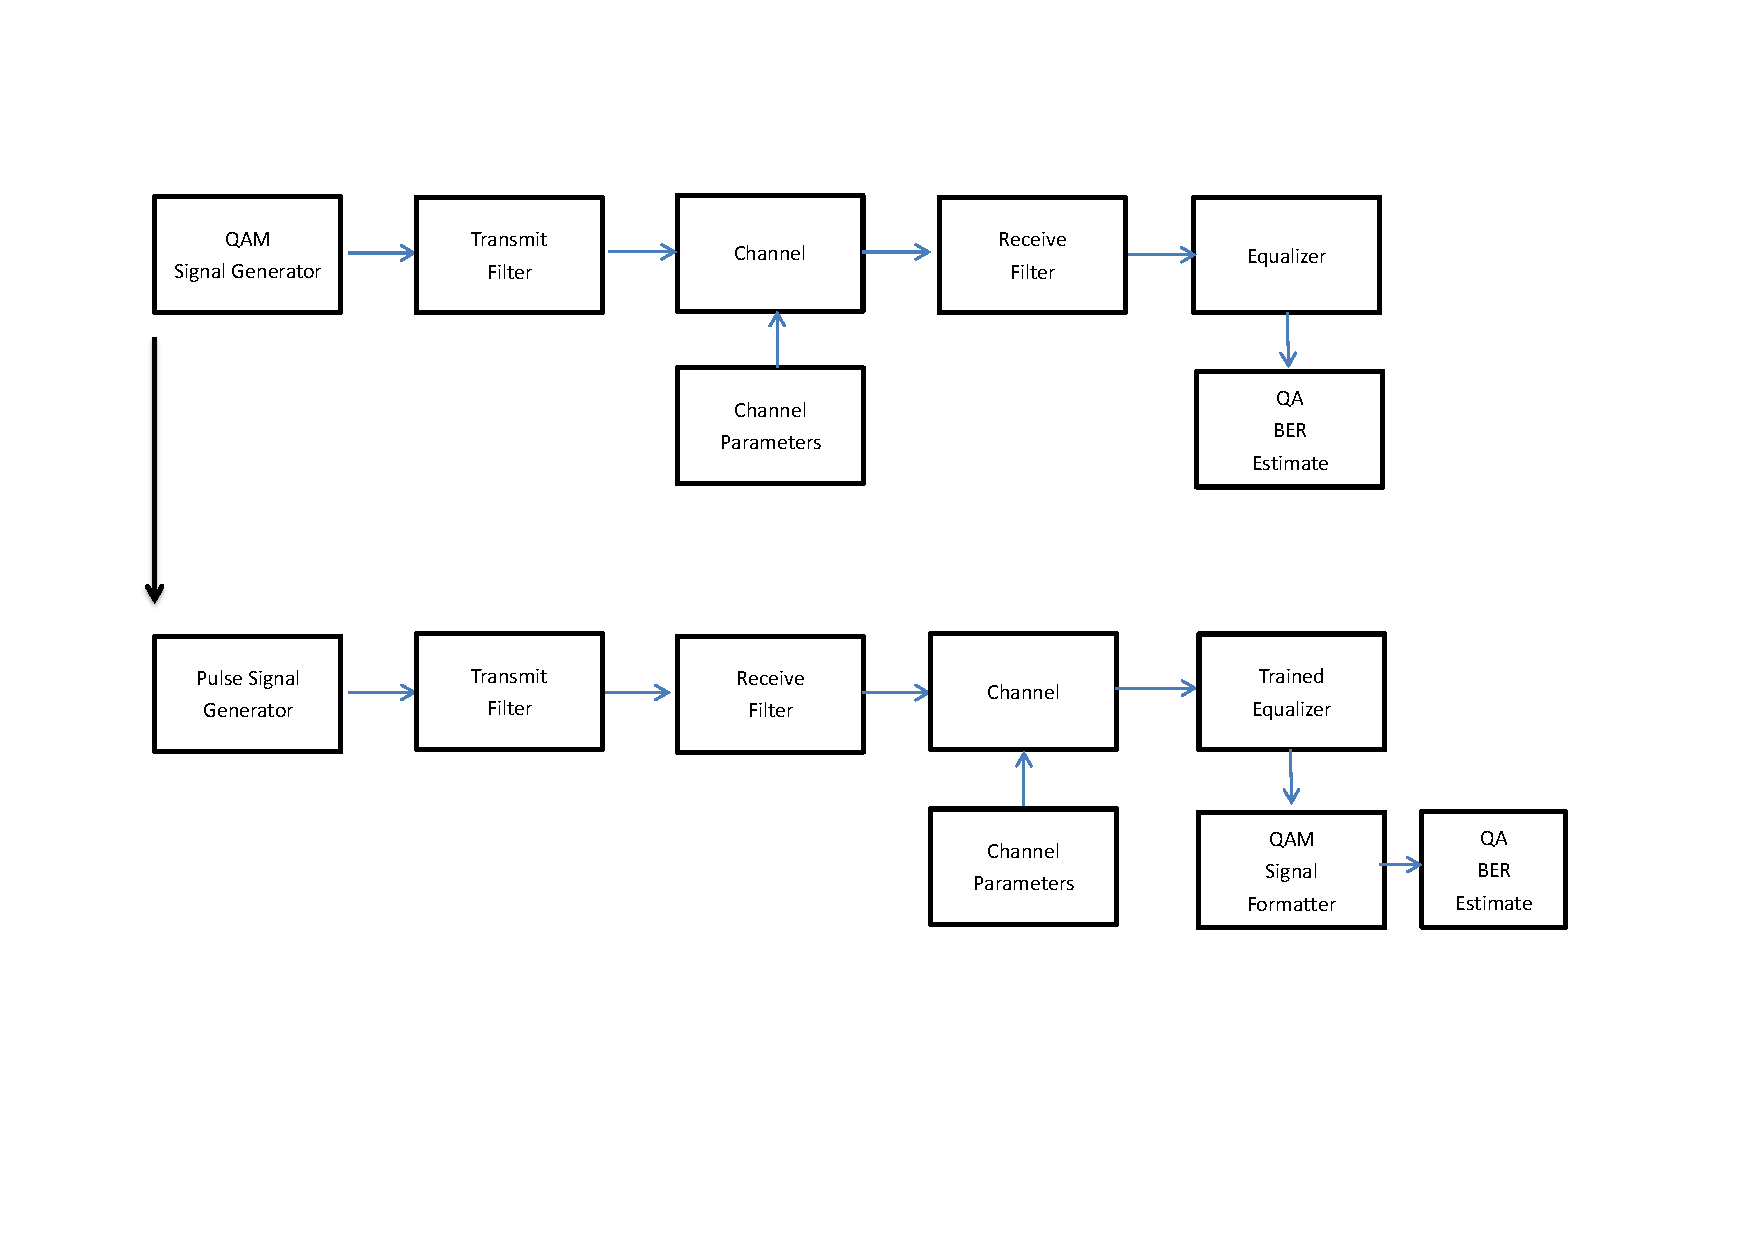
\includegraphics[scale=0.75,angle=90]{MonteCarlo001.pdf}
\caption{一个复杂系统框图的例子}\label{EvolutionofMonteCarloSimulation}
\end{figure}

\begin{figure}
[htbp]
\centering
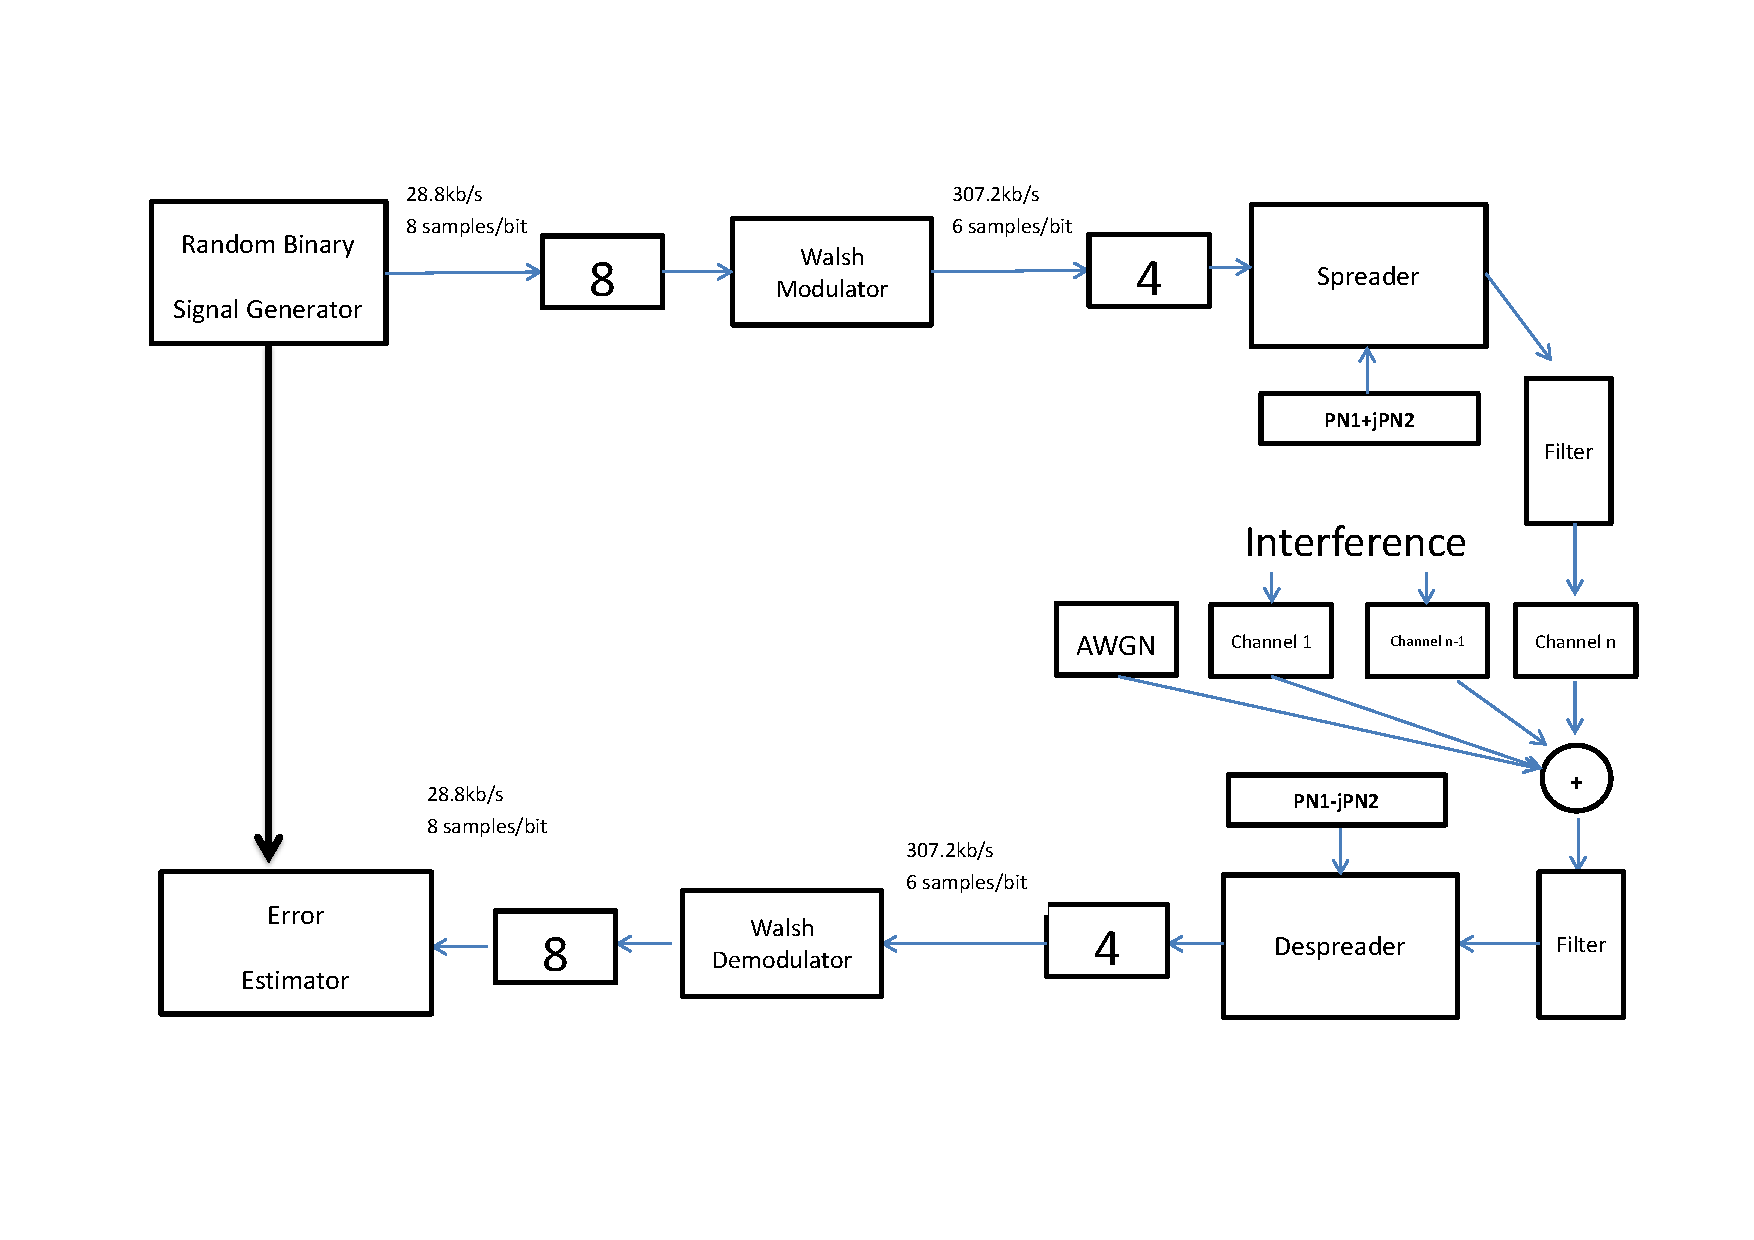
\includegraphics[scale=0.75,angle=90]{MonteCarlo002.pdf}
\caption{另一个复杂系统框图的例子}\label{BlockDiagramofReverseRadioLinkSimulation}
\end{figure}
建立好所需系统的模拟框图之后,在模拟软件(本文采用的是\upcite{MATLAB})里把每一个功能框都用对应的算法表示、代码实现出来。
蒙特卡罗方法的一个好处是不需要知道系统真实的输入信号---它将假定一个数字信号源作为输入。这样一来该方法便能很方便地比较
输入和输出之间的误差,从而得出有关系统性能的若干结论。
\par
对于本节讨论以及下一章部分计算采用的框图\ref{CommunicationSystemBlockDiagram}来说,其中一个很重要的部件(component)就是
系统的延时(delay)。由参考文献\upcite{Tranter1994,Ziemer1998}可知,讨论该系统(框图)的延时等同于讨论信号同步(synchronization)的问题。
对于载波调制(carrier-modulated)的信号做输入量系统来说,信号解调的问题和信号同步的问题是一回事。限于本文主旨和篇幅,
不做过多讨论。

\section{准分析方法}
准分析信道评估方法,也叫半解析(semianalytical)方法,是一种结合了系统模拟和纯数学推理计算的方法。这样一种方法
可以让系统的输出信号几乎完全消除噪声的干扰\upcite{Tranter1994}。该方法的描述如下,需要已知含有噪声的输出信号,并假定
噪声是已知概率密度函数(probability density function)的加性噪声。由于在处理时假定噪声的概率密度函数已知,我们可以很方便
地对输出端噪声的概率进行计算,这是数学推理的部分。在系统模拟部分,同样由于假定已知噪声的概率密度函数,我们可以在计算机
模拟的时候人工移除噪声的影响(MATLAB代码实现\upcite{Paul2011})。一个简明的准分析方法如图
\ref{IllusofQuasianalyticalMethod} 所示。
\begin{figure}
[htbp]
\centering
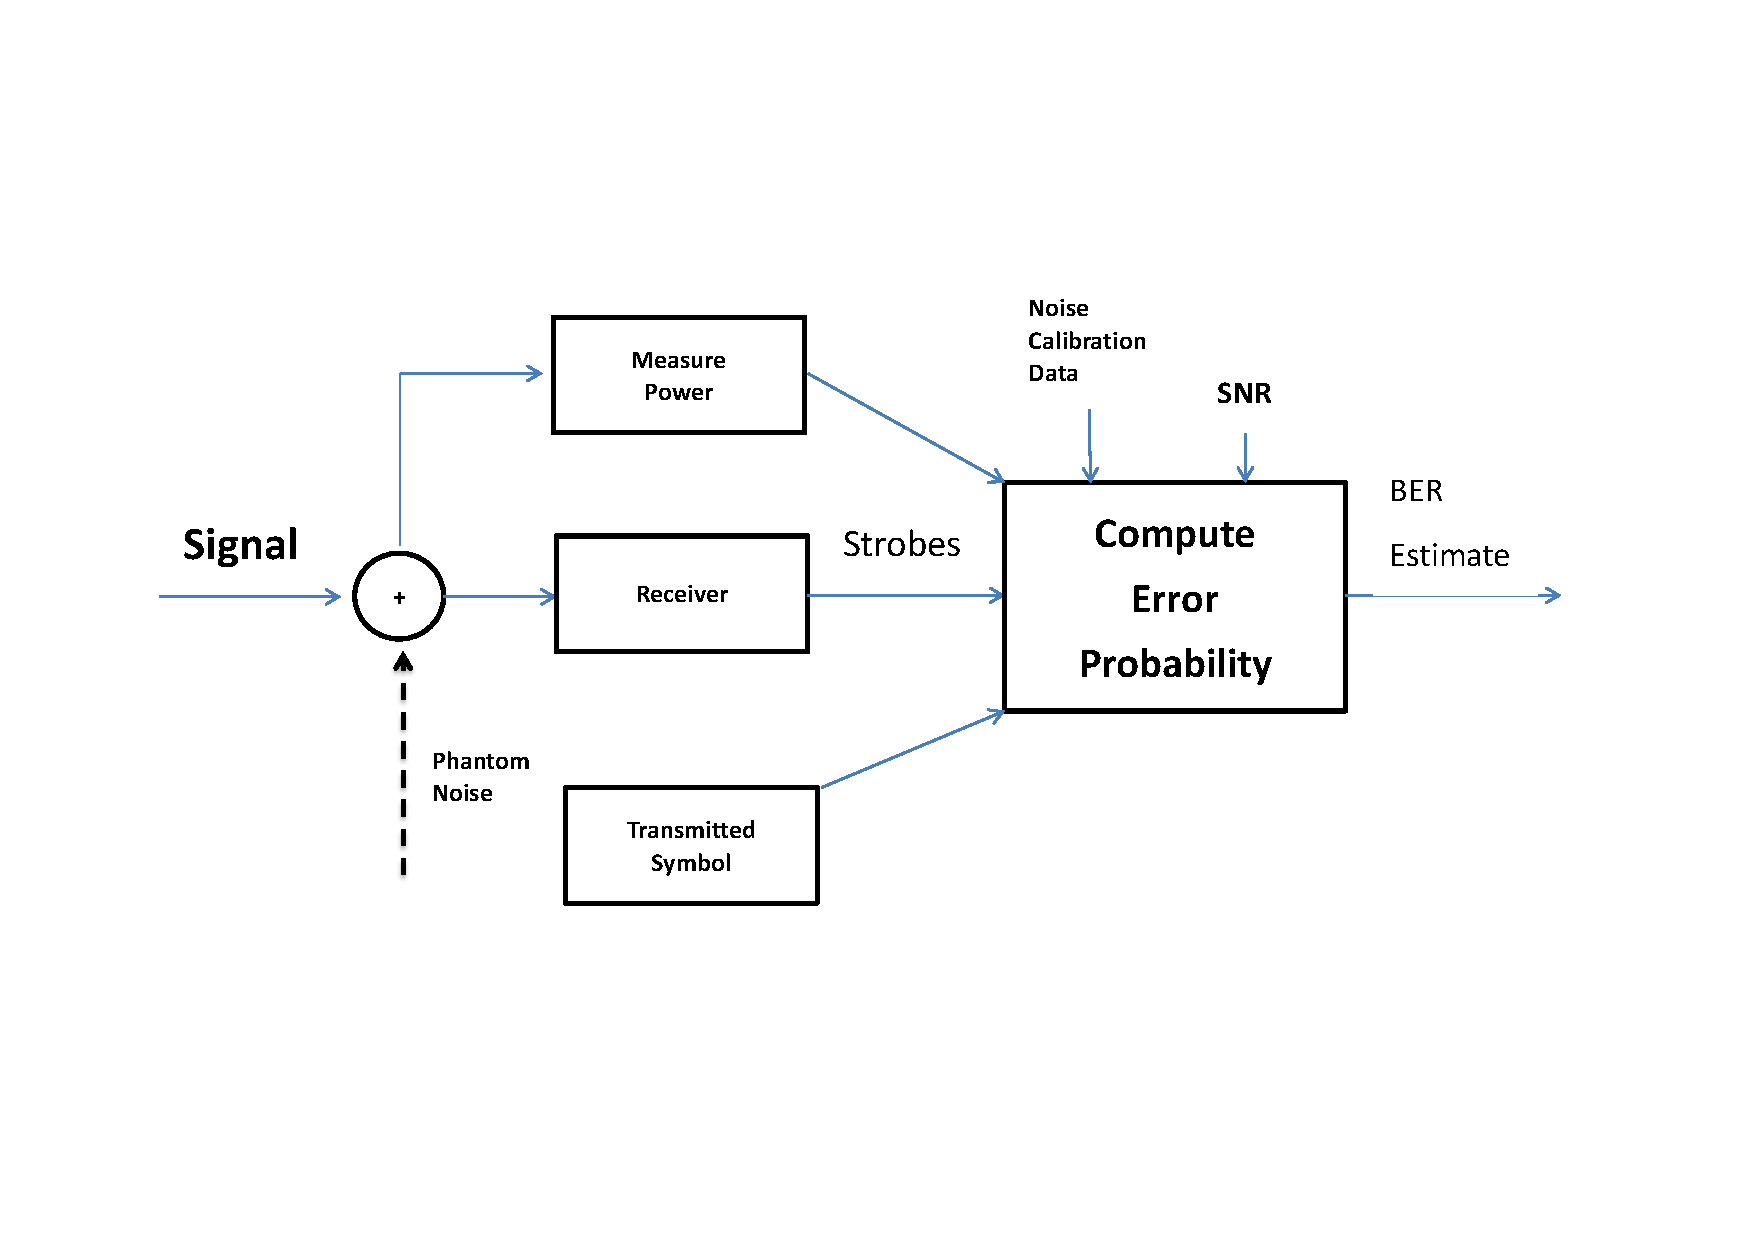
\includegraphics[scale=0.75,angle=90]{MonteCarlo003.pdf}
\caption{准分析方法框图示例}\label{IllusofQuasianalyticalMethod}
\end{figure}
该图的上半部分(a)表示的是一个假定的传输比特流,下半部分(b)表示的是去掉噪声后的接收机输入信号(即等待接收机
进行处理的信号)。现结合准分析方法对该图进行讨论。如果用符号$\nu_{k}$表示第$k$个采样瞬间对应的信号的幅值(即
纵坐标的数值),当考虑加性噪声时,可以将每个采样瞬间误差的概率用方程\ref{QuasiAnaResultingErrorProb}表示
\upcite{Tranter1994,Jeruchim2000,Ziemer1998}
\begin{equation}\label{QuasiAnaResultingErrorProb}
    P_{e_{k}}~=~
    \begin{cases}
    \displaystyle{Prob[noise>\nu_{k}]=\int^{\infty}_{\nu_{k}}f_{n}dn}, & \nu_{k}<0 \\
    \displaystyle{Prob[noise<\nu_{k}]=\int^{\nu_{k}}_{-\infty}f_{n}dn}, & \nu_{k}>0
    \end{cases}
\end{equation}
其中$f_{n}$表示的是在处理中假定已知加性噪声的的概率密度函数,并且其平均值(即概率密度函数的
数学期望)为了计算方便,假定为$0$。这一假定使得在本次讨论中信号相关检测解调的阈值(threshold)也为$0$。

\chapter{信道评估结果及分析}
本文仿真所用的代码由于较长,附在了附录里面。为了便于读者直观的分析、比较仿真结果,
所得的一共16张图片均作为正文放在了本章。
\section{仿真结果}
\begin{figure}[htbp]
  % Requires \usepackage{graphicx}
  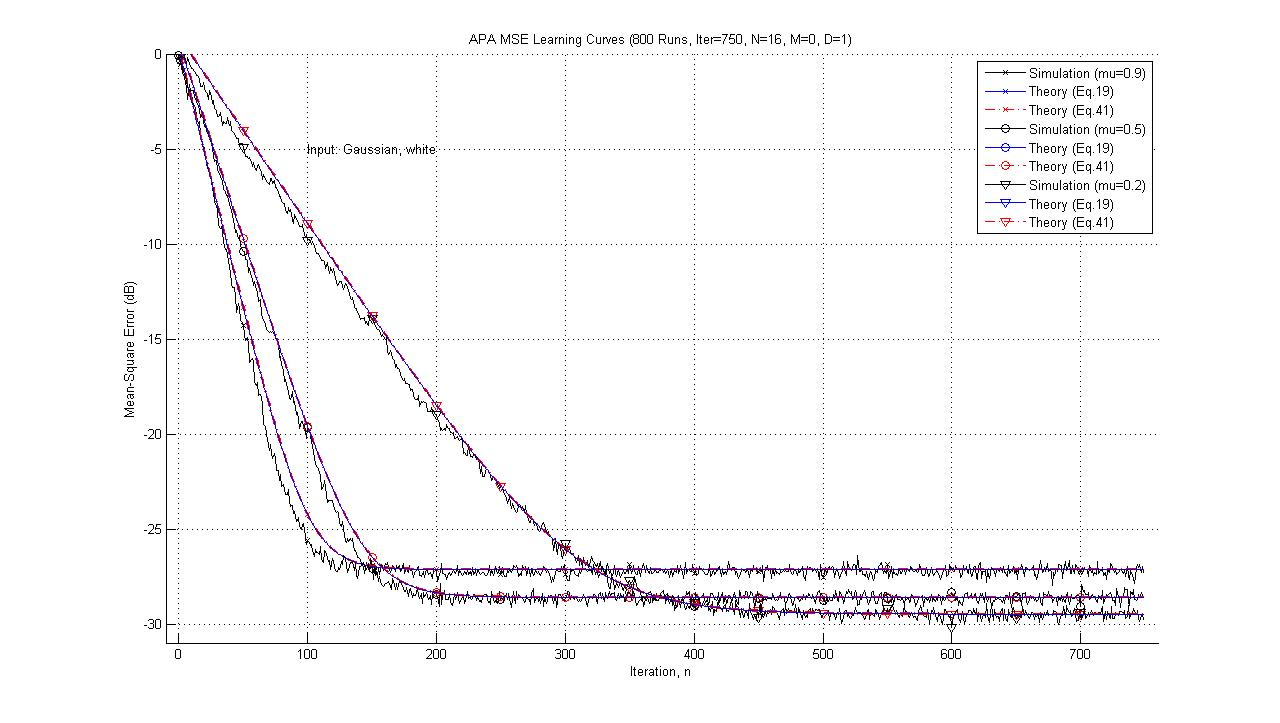
\includegraphics[scale=0.35]{Result001}\\
  \caption{APA MSE Learning Curves, 800 Runs, Iter=750, N=16, M=0, D=1}\label{APAMSE001}
\end{figure}

\begin{figure}[htbp]
  % Requires \usepackage{graphicx}
  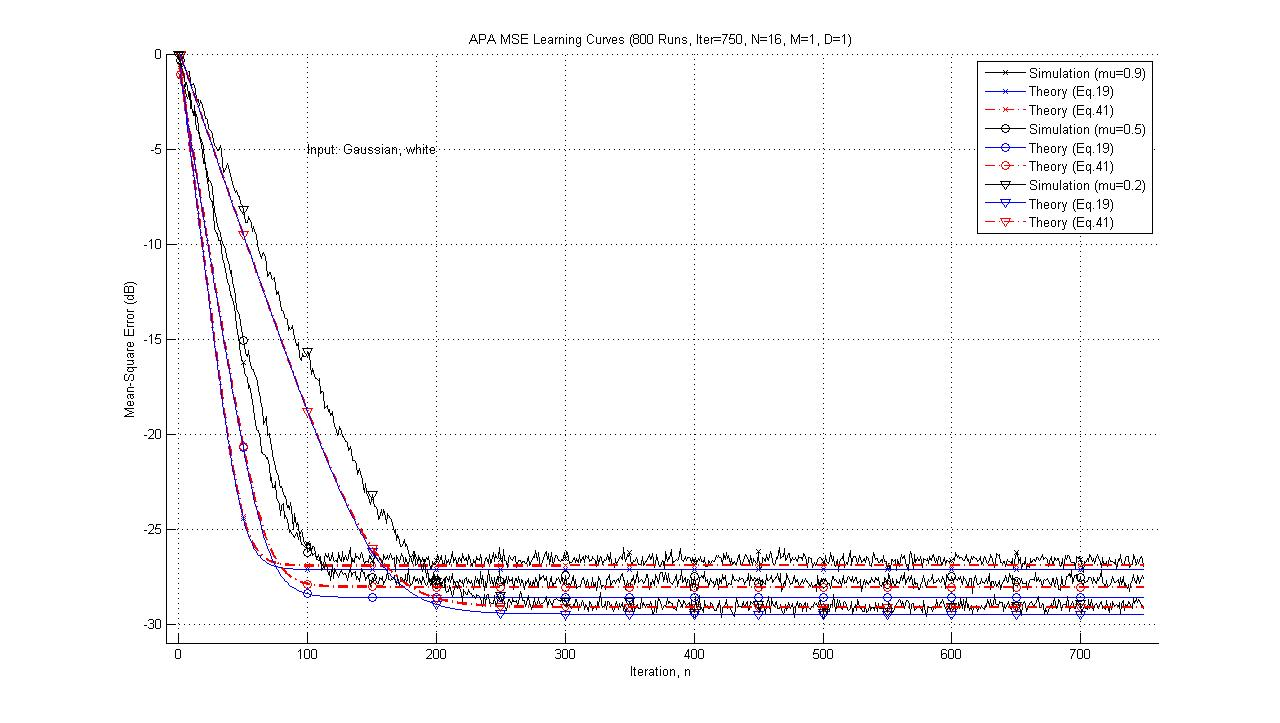
\includegraphics[scale=0.35]{Result002}\\
  \caption{APA MSE Learning Curves, 800 Runs, Iter=750, N=16, M=1, D=1}\label{APAMSE002}
\end{figure}

\begin{figure}[htbp]
  % Requires \usepackage{graphicx}
  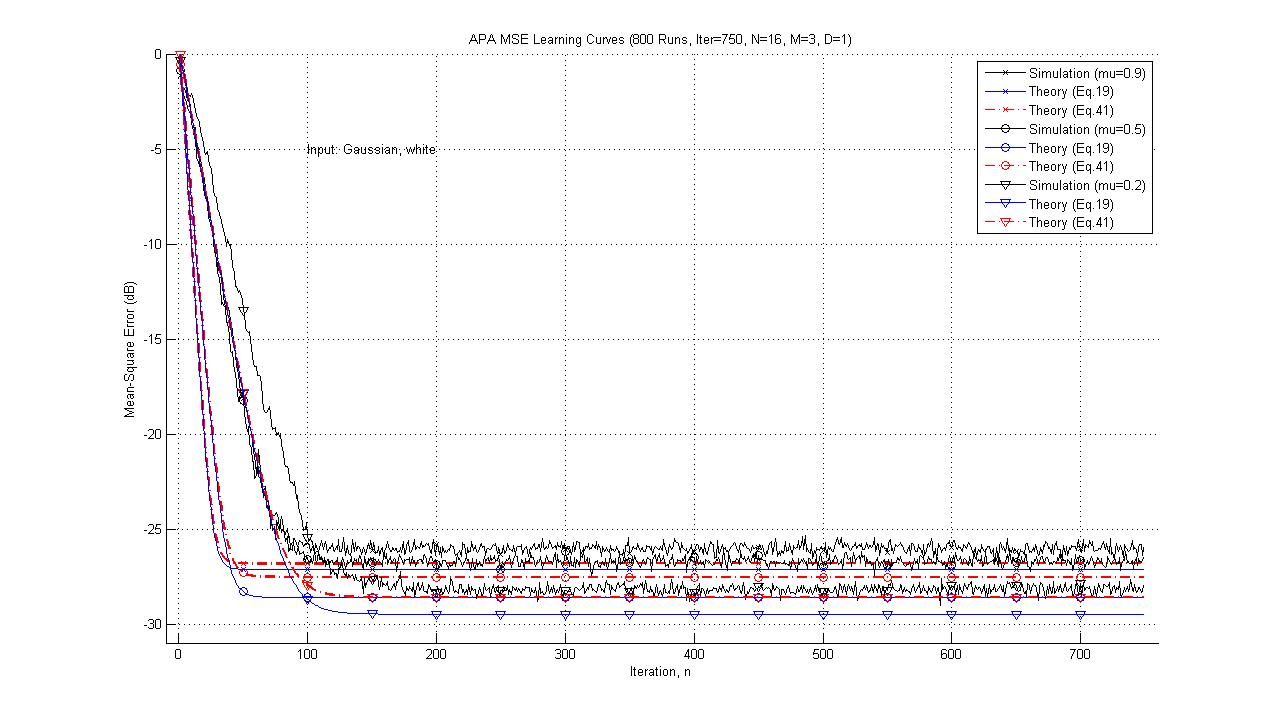
\includegraphics[scale=0.35]{Result003}\\
  \caption{APA MSE Learning Curves, 800 Runs, Iter=750, N=16, M=3, D=1}\label{APAMSE003}
\end{figure}

\begin{figure}[htbp]
  % Requires \usepackage{graphicx}
  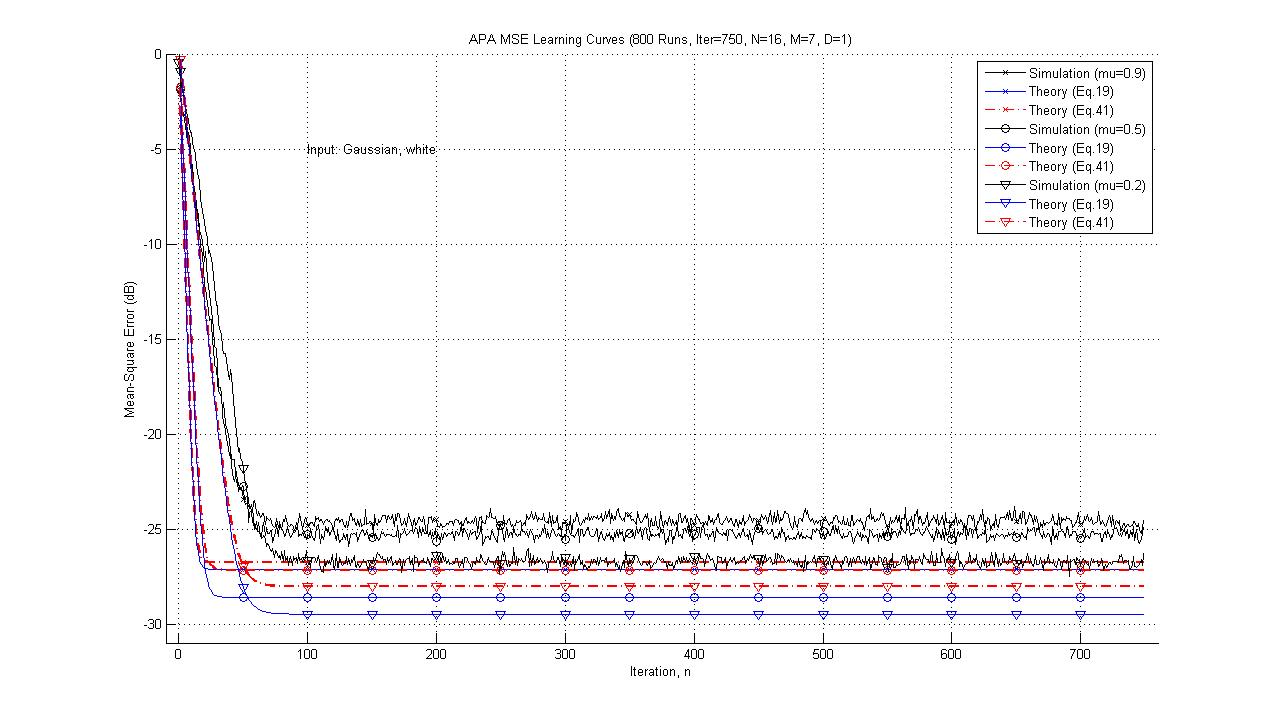
\includegraphics[scale=0.35]{Result004}\\
  \caption{APA MSE Learning Curves, 800 Runs, Iter=750, N=16, M=7, D=1}\label{APAMSE004}
\end{figure}

\begin{figure}[htbp]
  % Requires \usepackage{graphicx}
  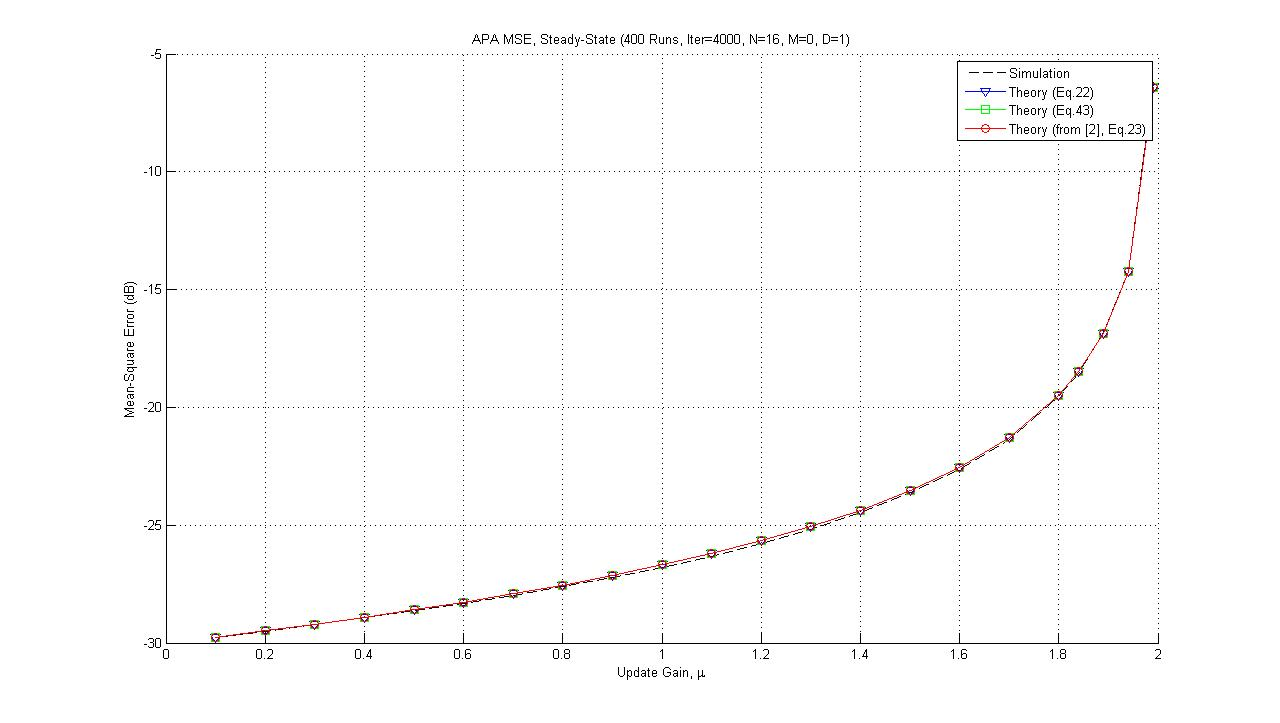
\includegraphics[scale=0.35]{Result005}\\
  \caption{APA MSE Steady State, 400 Runs, Iter=4000, N=16, M=0, D=1}\label{APAMSE005}
\end{figure}

\begin{figure}[htbp]
  % Requires \usepackage{graphicx}
  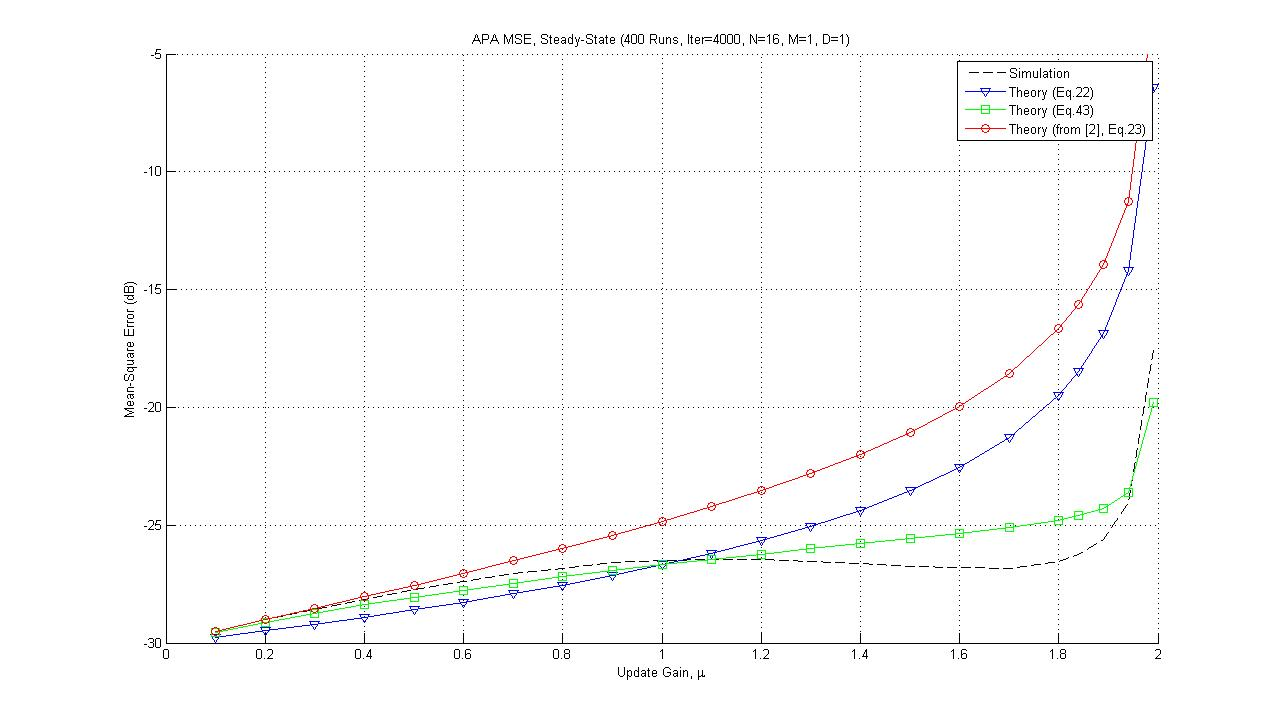
\includegraphics[scale=0.35]{Result006}\\
  \caption{APA MSE Steady State, 400 Runs, Iter=4000, N=16, M=1, D=1}\label{APAMSE006}
\end{figure}

\begin{figure}[htbp]
  % Requires \usepackage{graphicx}
  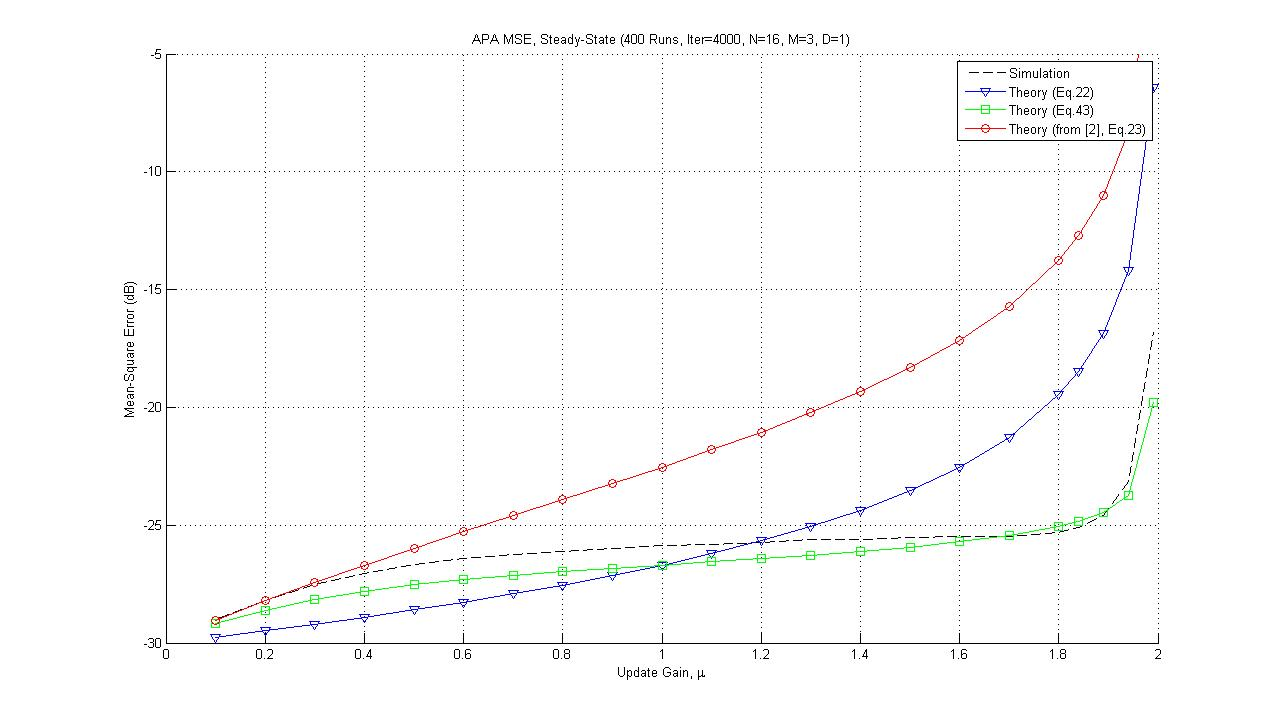
\includegraphics[scale=0.35]{Result007}\\
  \caption{APA MSE Steady State, 400 Runs, Iter=4000, N=16, M=3, D=1}\label{APAMSE007}
\end{figure}

\begin{figure}[htbp]
  % Requires \usepackage{graphicx}
  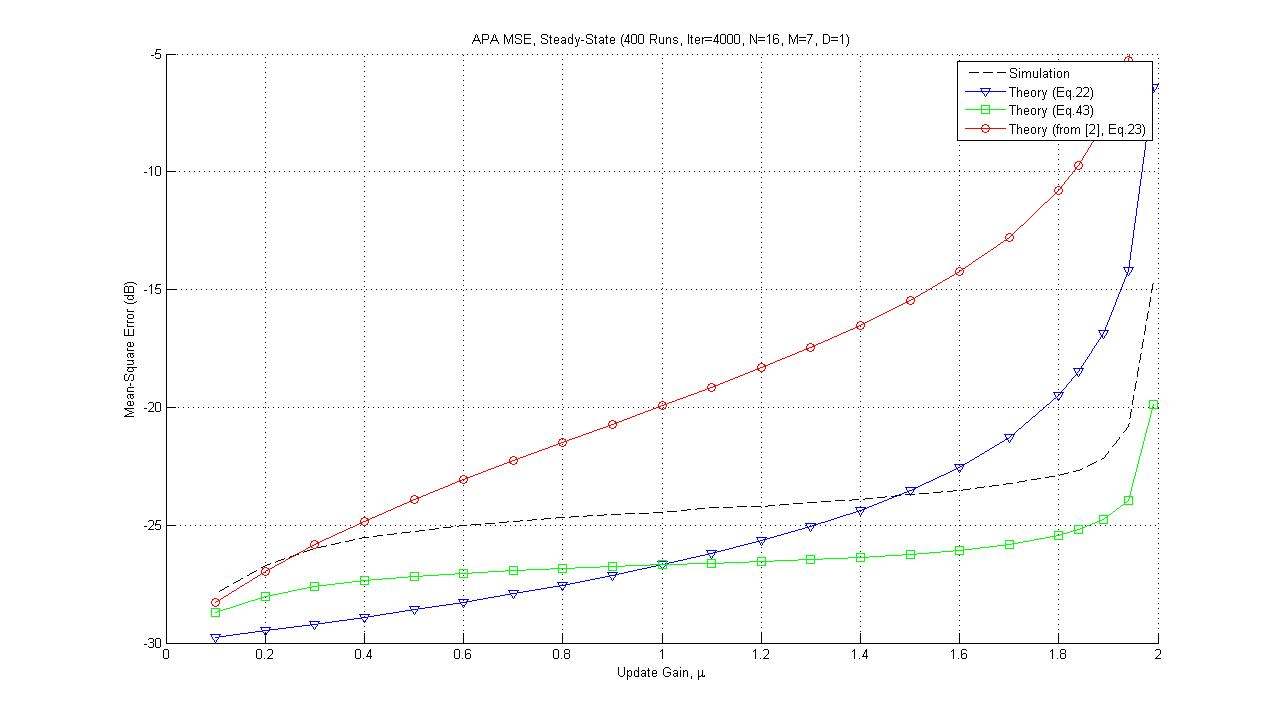
\includegraphics[scale=0.35]{Result008}\\
  \caption{APA MSE Steady State, 400 Runs, Iter=4000, N=16, M=7, D=1}\label{APAMSE008}
\end{figure}

\begin{figure}[htbp]
  % Requires \usepackage{graphicx}
  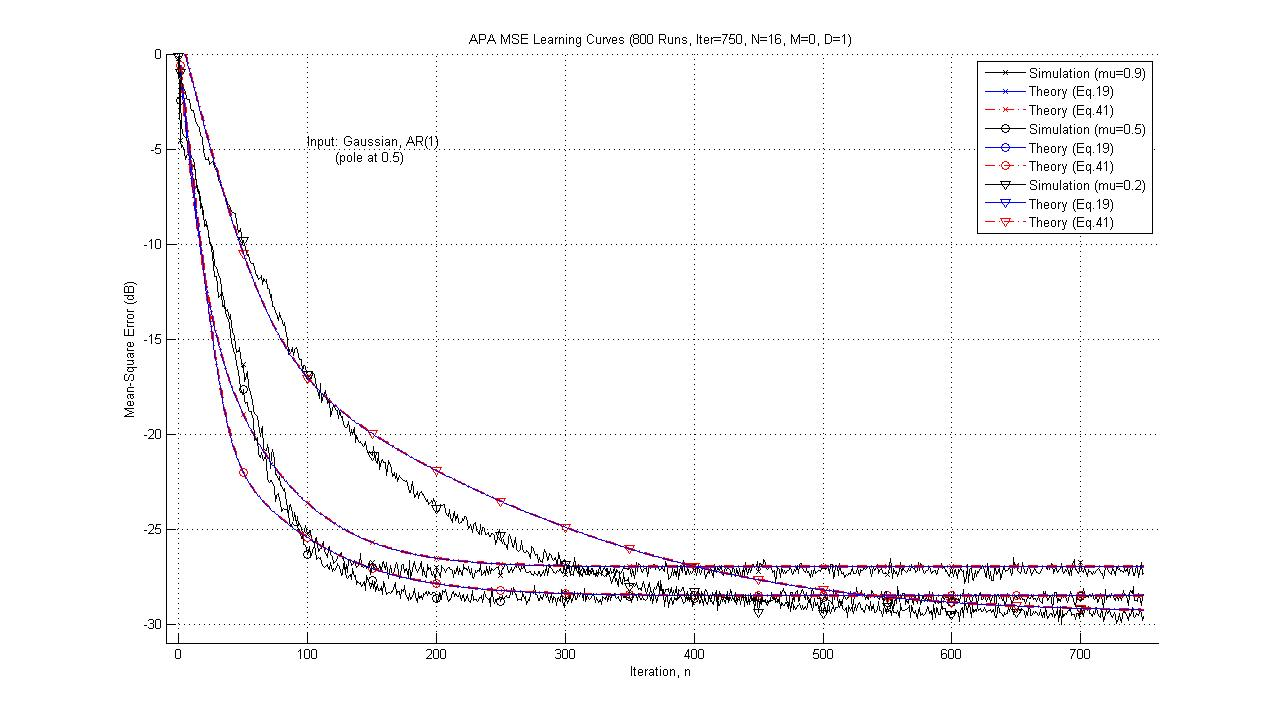
\includegraphics[scale=0.35]{Result009}\\
  \caption{APA MSE Learning Curve, 800 Runs, Iter=750, N=16, M=0, D=1}\label{APAMSE009}
\end{figure}

\begin{figure}[htbp]
  % Requires \usepackage{graphicx}
  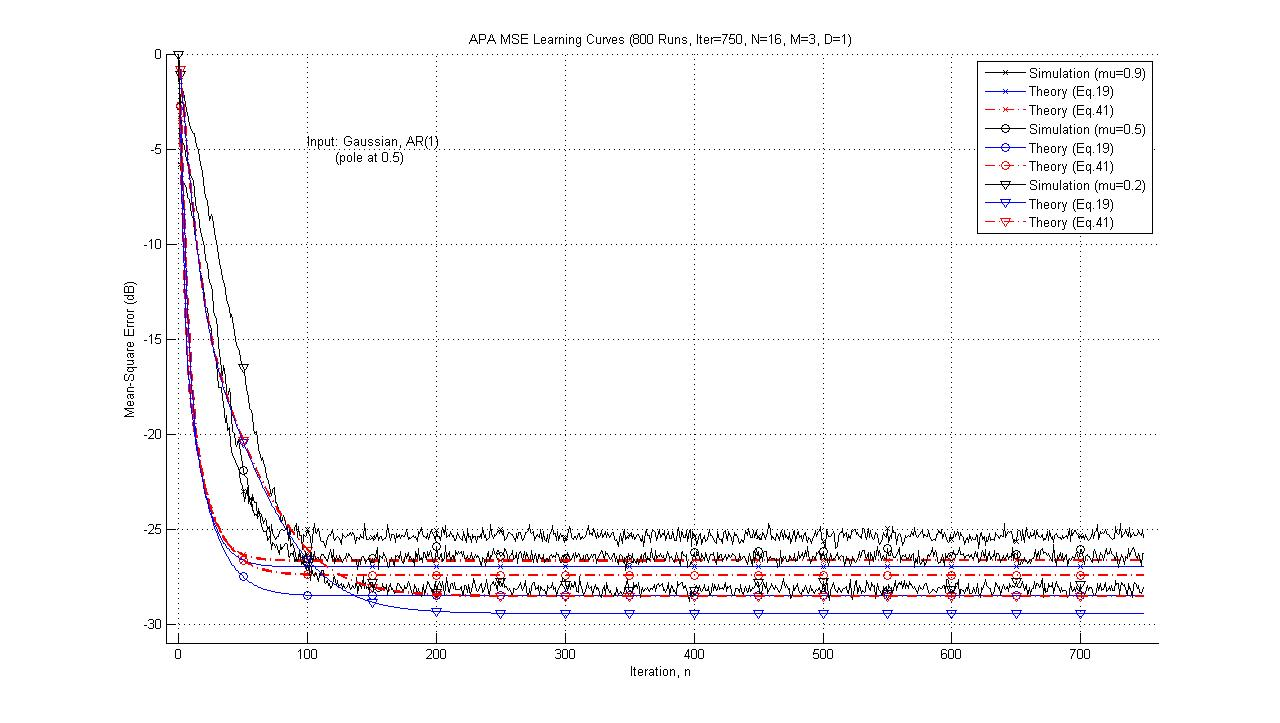
\includegraphics[scale=0.35]{Result010}\\
  \caption{APA MSE Learning Curve, 800 Runs, Iter=750, N=16, M=3, D=1}\label{APAMSE010}
\end{figure}

\begin{figure}[htbp]
  % Requires \usepackage{graphicx}
  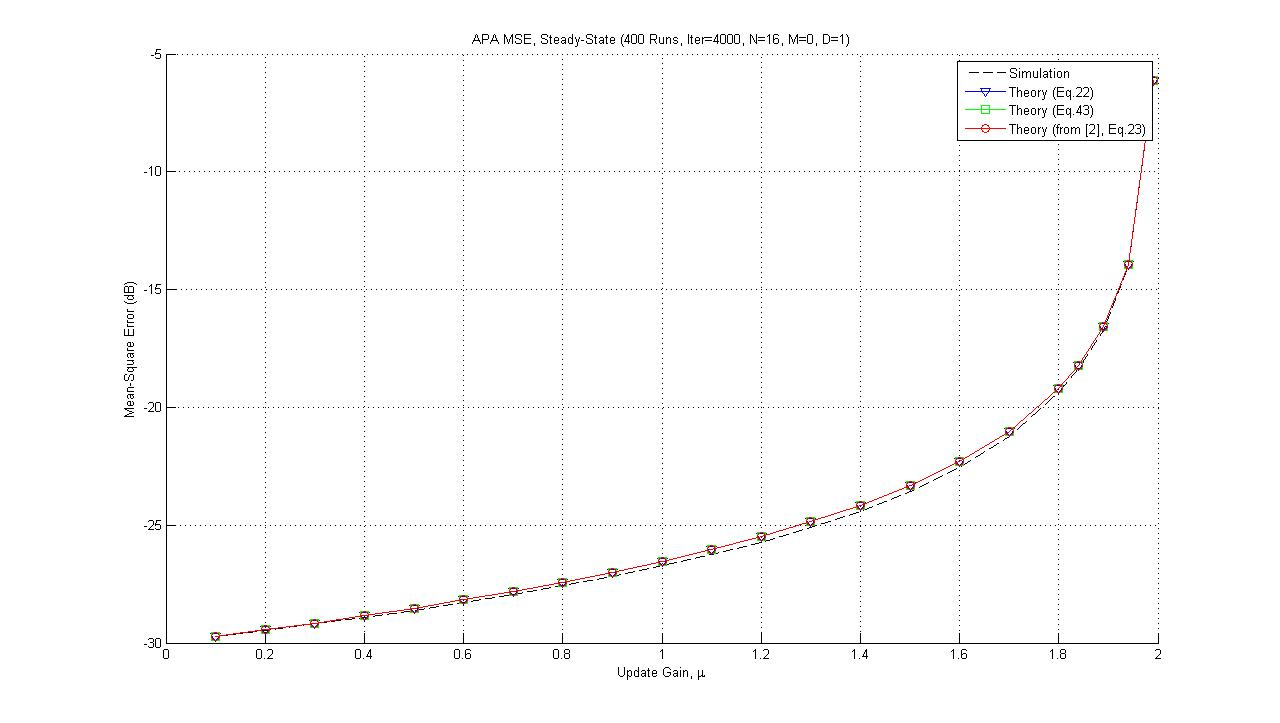
\includegraphics[scale=0.35]{Result011}\\
  \caption{APA MSE Steady State, 400 Runs, Iter=4000, N=16, M=0, D=1}\label{APAMSE011}
\end{figure}

\begin{figure}[htbp]
  % Requires \usepackage{graphicx}
  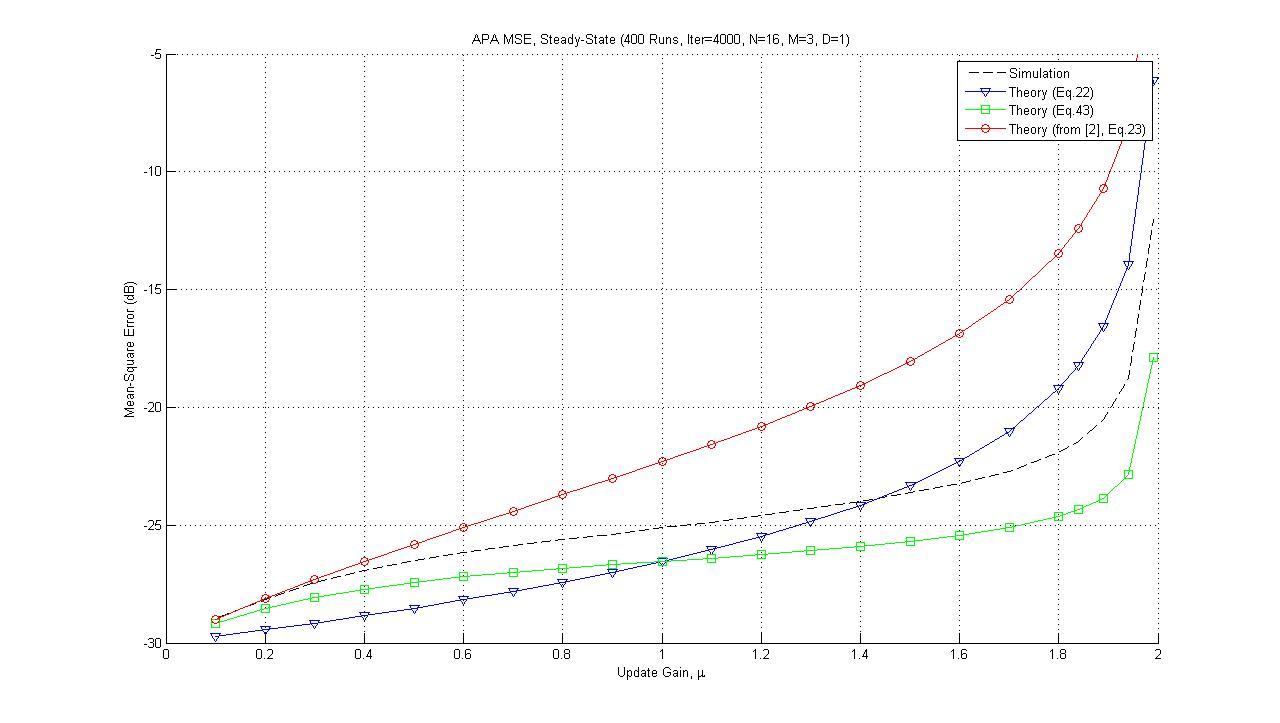
\includegraphics[scale=0.35]{Result012}\\
  \caption{APA MSE Steady State, 400 Runs, Iter=4000, N=16, M=3, D=1}\label{APAMSE012}
\end{figure}

\begin{figure}[htbp]
  % Requires \usepackage{graphicx}
  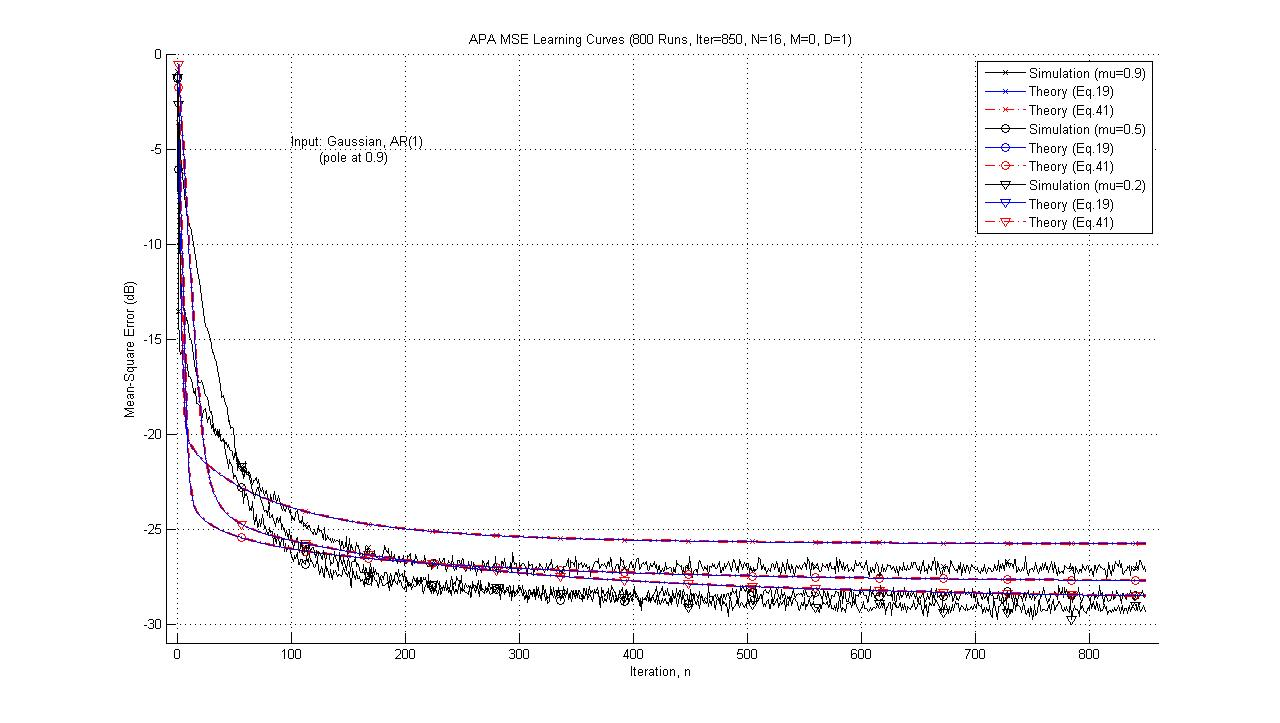
\includegraphics[scale=0.35]{Result013}\\
  \caption{APA MSE Learning Curve, 800 Runs, Iter=850, N=16, M=0, D=1}\label{APAMSE013}
\end{figure}

\begin{figure}[htbp]
  % Requires \usepackage{graphicx}
  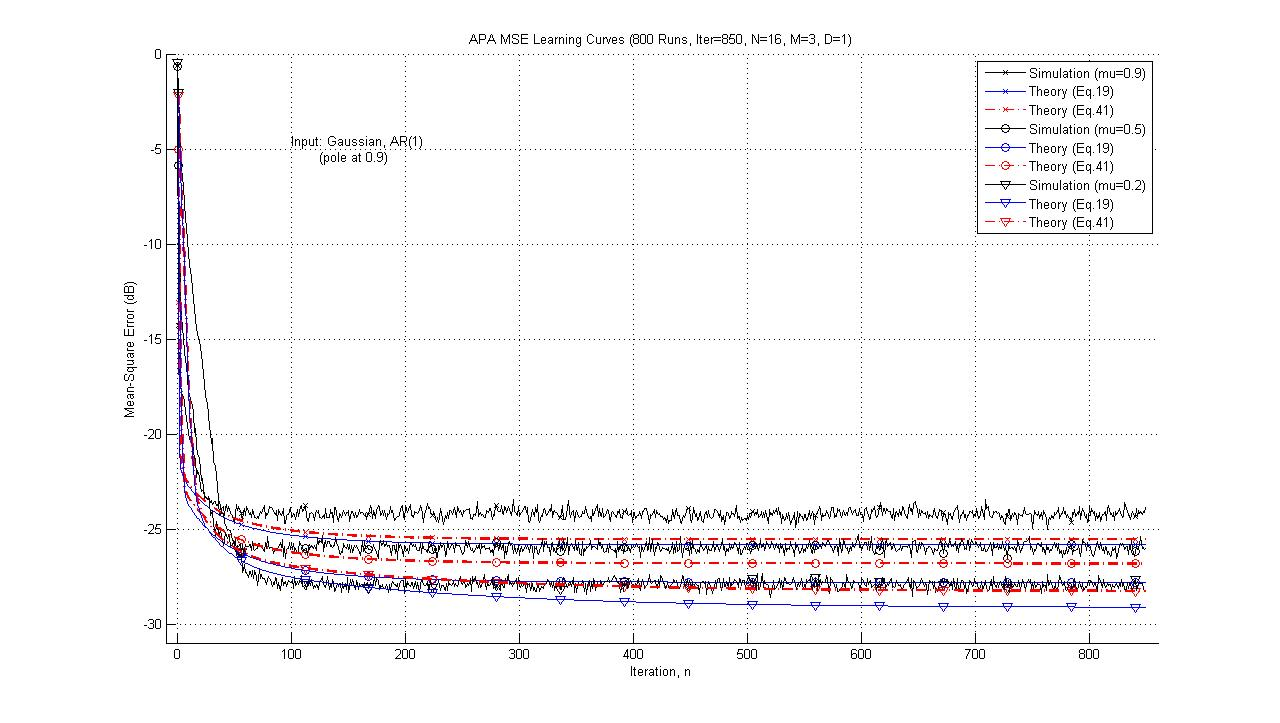
\includegraphics[scale=0.35]{Result014}\\
  \caption{APA MSE Learning Curve, 800 Runs, Iter=850, N=16, M=3, D=1}\label{APAMSE014}
\end{figure}

\begin{figure}[htbp]
  % Requires \usepackage{graphicx}
  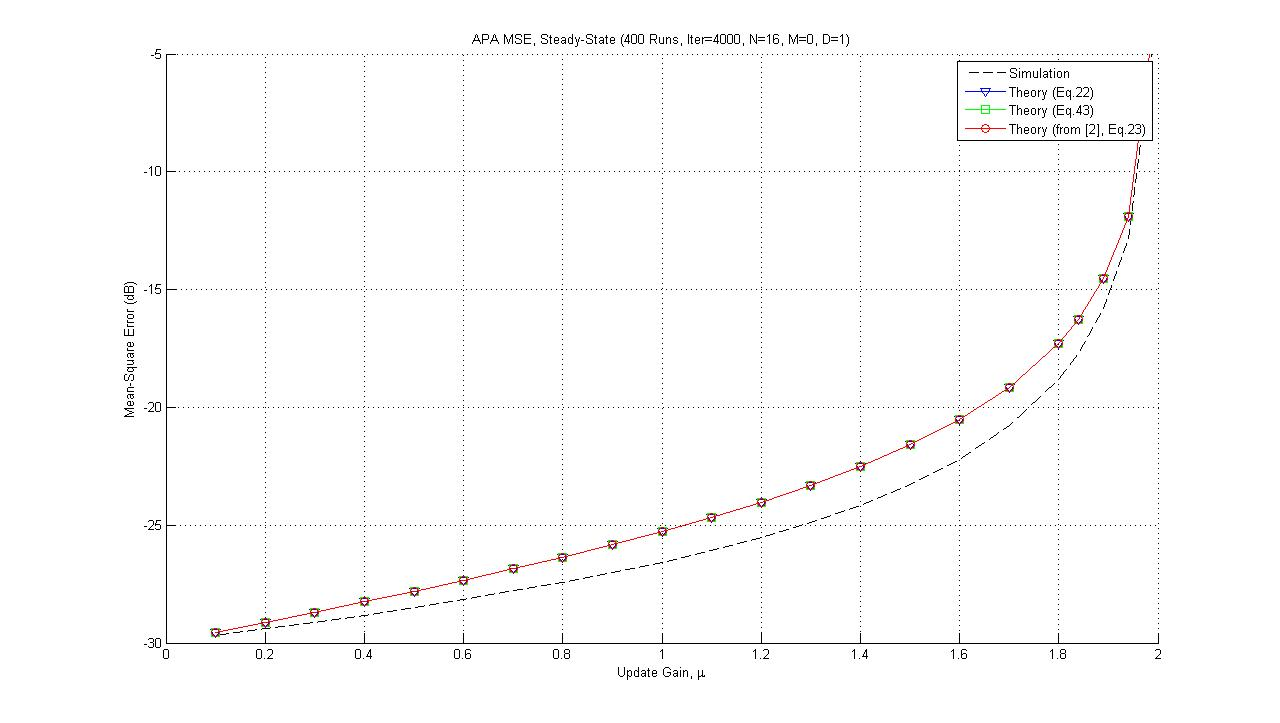
\includegraphics[scale=0.35]{Result015}\\
  \caption{APA MSE Steady State, 400 Runs, Iter=4000, N=16, M=0, D=1}\label{APAMSE015}
\end{figure}

\begin{figure}[htbp]
  % Requires \usepackage{graphicx}
  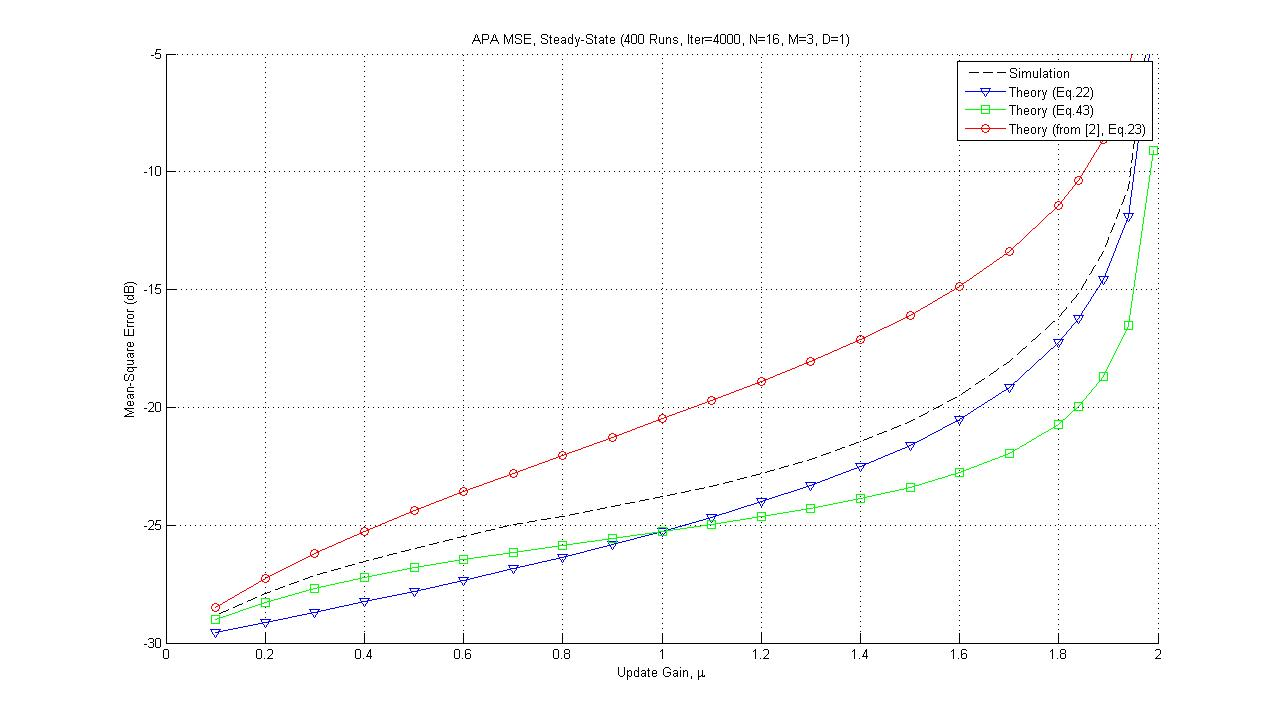
\includegraphics[scale=0.35]{Result016}\\
  \caption{APA MSE Steady State, 400 Runs, Iter=400, N=16, M=3, D=1}\label{APAMSE016}
\end{figure}
\section{结果分析}
现在根据上节所列的仿真结果对全文做一个总结。基于仿射投影算法的自适应滤波器,在最小均方滤波器家族中
有着比归一化最小均方滤波器更好的收敛程度,因此在计算复杂度不是主要考虑因素的前提下,仿射投影自适应滤波器
是一个很好的选择---如前所述,介于两个极端,归一化最小均方和递归最小均方两个极端之间。
\begin{itemize}
  \item 仿射投影自适应滤波器的学习曲线包含有指数项求和的运算,因此有一定的计算复杂度。
  \item 仿射投影自适应滤波器的收敛速度比归一化最小均方滤波器要快,因此能经过较少次
  的迭代而获得期望结果。
  \item 当滤波器的阶数$N$增加的时候,在迭代时可以用的输入数据矢量$\mathbf{u}_{n}$也随之增多。从理论
  和仿真两方面均证明了这样收敛性会变得更好,不过收敛速率却随之降低。
\end{itemize}
总的来说,通信系统的设计和评估领域有这样一句脍炙人口的话,可以很好地作为全篇的一个总结,“设计通信系统
的时候没有免费的午餐可以吃,对于我们取得的每一分贝增益,我们都付出了等额的代价。”(\emph{There is no
free lunch in designing a communication system: for every gain that is made, there is a price to be
paid.})

% Bibliography
\bibliographystyle{unsrt}
\bibliography{contents/reference}
\addcontentsline{toc}{chapter}{参考文献}

\chapter*{致\quad谢}
\addcontentsline{toc}{chapter}{致谢}
本文从开题之初到设计实验、完成实验和论文撰写,及至今日在这里做最后的答辩工作,得到了很多同学与老师的帮助与支持。
现一一感谢如下。
\par
首先要感谢的就是我的指导老师智永锋。我在大四上学期完成所有课程之后就开始联系可能加入团队并进行毕业设计的老师们,
譬如洪亮老师和张慧翔老师。在和智老师的沟通当中,他详细地介绍了所在课题组目前主力从事的一项国家自然科学基金研究,
并表示我在该领域的研究成果将对日后的深造产生深远影响---因为做的是很基础的东西。在毕业设计进行的过程当中,智老师
坚持每周至少一次的会谈,对我工作的进度和遇到的困难嘘寒问暖。信号领域的基础研究,对数学的要求极高,在有我看不懂
的公式的时候,智老师会带着我从头把公式推一遍,这也是为什么各位老师能够看到一篇有很多公式和推演的文章;由于我所在
的专业对MATLAB实践能力的要求并不高,在我温习MATLAB的时候,有不懂的问题,一封电子邮件过去之后我
过十几分钟就能收到很详尽的阐述,甚至附带了几篇相关的文章要求我阅读。智老师也是我出国留学推荐信的撰写人之一,能在
大学的最后一段时间内把标准提到硕士研究生的水平,我想正是为我日后的科学研究道路在做准备吧!
\par
本学期刚开学,我就向老师申请并顺利加入了自动化学院511教研室。在今年这一批研究生快要毕业的时候,我聆听了
他们的预答辩,这给我准备现在的答辩提供了很大的帮助;在平时与研究生师兄师姐一起工作的时候,我能用我扎实的
计算机科学功底帮助他们解决一些问题,也能从他们身上提早知道科研道路的艰辛与做出成果之后的开心。
\par
在本文作者进行开题报告答辩的时候,唐伟教授和曲仕茹教授对本人提出的设计思路,依据他们多年科研领域的工作经验,
进行了有效的质疑。这让本人在后面几个月少走了很多弯路,在此一并感谢。
\par
本人算班级体里面的“捣蛋分子”了。在进行毕业设计、论文撰写的过程当中,偶尔由于进度和工作量的压力太大,
对同学们进行了轻微的骚扰,他们也都表示理解和接受,一并感谢。
\par
最后,但并不是最不重要的,我想感谢我的父母。大家都知道没有父母亲就没有我们这个道理,但是我是那种怎么着也找不到
女朋友的孩子,因此为了克服每天对着不是书本就是笔记本(计算机)的苦楚,本人基本上每天要给家里去一个电话,跟爸爸或者
妈妈谈谈心,汇报一下自己每天的工作和经验教训。在学术领域父母加起来可能还是没有我懂得多,也没有我在业务上这么熟练;
但是在生活领域,我是彻头彻尾的小菜鸡,我想这也是同学眼力“学霸”不为人知的一面吧---没有父母亲背后数十年如一日
的支持,我想我早就退出科研领域,回老家安安稳稳过一辈子去了。

\chapter*{毕业设计小结}
\addcontentsline{toc}{chapter}{小结}
如果毕业设计的全过程仅仅是按照开题报告的要求,把该做的做出来,把该写的东西写好,那么我想教务部门
也没有必要搞一个“小结”放在最后了,直接重新看一下我们的开题报告和摘要不就好了。他们需要用来评判的全部
东西都在那里了。之所以需要我们撰写这一部分,我认为老师们是想了解更多幕后的事情。
\par
真要写,这里也能写个成千上万字,毕竟是大学的最后一个学期了么,毕竟这个学期没有课程的安排,彻彻底底的回到
时间由我们自由支配的“理想化状态”了。我在2013年3月份的时候去美国的一个网站申请了虚拟主机和自己的顶级域名
\footnote{\url{http://abrahamx.com}},计划的就是从这个完全自由的学期开始把重要的东西记录下来,现在按照
时间顺序和重要程度展示一点,我为自己的研究生生涯做的努力和准备吧。
\begin{itemize}
  \item \textbf{二月。}与指导老师就毕业设计的选题进行了进一步的沟通。对即将进行为期4个月的研究做了
  很深入的背景调研,手段是搜索引擎Google和与国外教授的电子邮件。
  \item \textbf{三月。}在不少时间浪费掉之后,重新意识到时间管理与目标控制的重要性,花大力气阅读了
  "Getting Things Done, The Art of Stress-Free Productivity",并因此很大程度提高了每天在教研室
  的工作效率。此外,还抽空阅读了《演讲之禅》与《黑客与画家》,对重新认识科研和商业领域有很大帮助。
  \item \textbf{四月。}在这个月集中攻坚了通信领域的理论基础。花很大的力气阅读并理解了"Signals and
  Systems", "Discrete-Time Signal Processing"和"Principles of Communications"三本麻省理工学院(MIT)
  的本科生教材。这打下了本文坚实的理论基础。
  \item \textbf{五月。}这个月从好友那里得知了一所很不错的只招研究生的学校的申请机会,并赶在
  截止日期之前与教授进行了沟通、做了申请。这个月的主要工作集中在设计前文所述的几个系统框图,
  并通过MATLAB编程对若干种设计思想进行了检验。
  \item \textbf{六月。}这个月完成了五月份开始的毕业设计论文撰写。并在指导老师智永锋的帮助下,对文章进行了
  修改和完善。此外,智老师校对了本人的英语翻译工作,还同样对答辩PPT提出了修改意见。
\end{itemize}
我的很多同学都选择了在国内继续接受硕士研究生的高等教育,我选择了一条更为艰辛的海外求学道路。正式接受Offer的学校
是\emph{Masdar Institute of Science and Technology},虽然在不为人知的阿布扎比,但是据一位今年
正式毕业的系工大校友介绍,学风和校风都很好---课程还很难。为此,我再一次感谢自己在这几个月里面养成的
刻苦钻研、博学审问的习惯。而这种习惯对于一个立志在学术界做出一番成就的准研究生来说,正是不可或缺的。




























































